\PassOptionsToPackage{unicode=true}{hyperref} % options for packages loaded elsewhere
\PassOptionsToPackage{hyphens}{url}
%
\documentclass[11pt,ignorenonframetext,]{beamer}
\usepackage{pgfpages}
\setbeamertemplate{caption}[numbered]
\setbeamertemplate{caption label separator}{: }
\setbeamercolor{caption name}{fg=normal text.fg}
\beamertemplatenavigationsymbolsempty
% Prevent slide breaks in the middle of a paragraph:
\widowpenalties 1 10000
\raggedbottom
\setbeamertemplate{part page}{
\centering
\begin{beamercolorbox}[sep=16pt,center]{part title}
  \usebeamerfont{part title}\insertpart\par
\end{beamercolorbox}
}
\setbeamertemplate{section page}{
\centering
\begin{beamercolorbox}[sep=12pt,center]{part title}
  \usebeamerfont{section title}\insertsection\par
\end{beamercolorbox}
}
\setbeamertemplate{subsection page}{
\centering
\begin{beamercolorbox}[sep=8pt,center]{part title}
  \usebeamerfont{subsection title}\insertsubsection\par
\end{beamercolorbox}
}
\AtBeginPart{
  \frame{\partpage}
}
\AtBeginSection{
  \ifbibliography
  \else
    \frame{\sectionpage}
  \fi
}
\AtBeginSubsection{
  \frame{\subsectionpage}
}
\usepackage{lmodern}
\usepackage{amssymb,amsmath}
\usepackage{ifxetex,ifluatex}
\usepackage{fixltx2e} % provides \textsubscript
\ifnum 0\ifxetex 1\fi\ifluatex 1\fi=0 % if pdftex
  \usepackage[T1]{fontenc}
  \usepackage[utf8]{inputenc}
  \usepackage{textcomp} % provides euro and other symbols
\else % if luatex or xelatex
  \usepackage{unicode-math}
  \defaultfontfeatures{Ligatures=TeX,Scale=MatchLowercase}
\fi
\usetheme[]{metropolis}
% use upquote if available, for straight quotes in verbatim environments
\IfFileExists{upquote.sty}{\usepackage{upquote}}{}
% use microtype if available
\IfFileExists{microtype.sty}{%
\usepackage[]{microtype}
\UseMicrotypeSet[protrusion]{basicmath} % disable protrusion for tt fonts
}{}
\IfFileExists{parskip.sty}{%
\usepackage{parskip}
}{% else
\setlength{\parindent}{0pt}
\setlength{\parskip}{6pt plus 2pt minus 1pt}
}
\usepackage{hyperref}
\hypersetup{
            pdftitle={Lecture 21},
            pdfauthor={Colin Rundel},
            pdfborder={0 0 0},
            breaklinks=true}
\urlstyle{same}  % don't use monospace font for urls
\newif\ifbibliography
\usepackage{longtable,booktabs}
\usepackage{caption}
% These lines are needed to make table captions work with longtable:
\makeatletter
\def\fnum@table{\tablename~\thetable}
\makeatother
\setlength{\emergencystretch}{3em}  % prevent overfull lines
\providecommand{\tightlist}{%
  \setlength{\itemsep}{0pt}\setlength{\parskip}{0pt}}
\setcounter{secnumdepth}{0}

% set default figure placement to htbp
\makeatletter
\def\fps@figure{htbp}
\makeatother

\usepackage{geometry}
\usepackage{graphicx}

\usepackage{bbold}
\usepackage{lmodern}


\usepackage{url}		% produces hyperlinks

\usepackage{colortbl}	% allows for color usage in tables
\usepackage{multirow}	% allows for rows that span multiple rows in tables

\usepackage{color}          	% gives color options
\usepackage{xcolor}		% this package has a variety of color options

\usepackage{multicol}
\usepackage{textcomp}

\usepackage{setspace}
\usepackage{changepage}
\usepackage{isotope}

\singlespacing

\def\begincol{\begin{column}}
\def\endcol{\end{column}}

\def\begincols{\begin{columns}}
\def\endcols{\end{columns}}

%%%%%%%%%%%%%%%%
% Small code output
%%%%%%%%%%%%%%%%

%% change fontsize of R code

\makeatletter
\@ifundefined{Shaded}{\newenvironment{Shaded}{}{}}{}
\makeatother


\let\oldShaded\Shaded
\let\endoldShaded\endShaded
\renewenvironment{Shaded}{\footnotesize\begin{spacing}{0.9}\oldShaded}{\endoldShaded\end{spacing}}

%% change fontsize of output
\let\oldverbatim\verbatim
\let\endoldverbatim\endverbatim
\renewenvironment{verbatim}{\footnotesize\begin{spacing}{0.9}\oldverbatim}{\endoldverbatim\end{spacing}}


\newcommand{\tinyoutput}{
  \renewenvironment{Shaded}{\tiny\begin{spacing}{0.9}\oldShaded}{\endoldShaded\end{spacing}}
  \renewenvironment{verbatim}{\tiny\begin{spacing}{0.9}\oldverbatim}{\endoldverbatim\end{spacing}}
}

\newcommand{\scriptoutput}{
  \renewenvironment{Shaded}{\scriptsize\begin{spacing}{0.9}\oldShaded}{\endoldShaded\end{spacing}}
  \renewenvironment{verbatim}{\scriptsize\begin{spacing}{0.9}\oldverbatim}{\endoldverbatim\end{spacing}}
}

\newcommand{\footnoteoutput}{
  \renewenvironment{Shaded}{\footnotesize\begin{spacing}{0.9}\oldShaded}{\endoldShaded\end{spacing}}
  \renewenvironment{verbatim}{\footnotesize\begin{spacing}{0.9}\oldverbatim}{\endoldverbatim\end{spacing}}
}

%\newcommand{\verbatimfont}[1]{\renewcommand{\verbatim@font}{\ttfamily#1}}


%%%%%%%%%%%%%%%%
% Custom Colors
%%%%%%%%%%%%%%%%

\definecolor{redhl}{rgb}{0.98,0.29,0.28}
\definecolor{yellowhl}{rgb}{0.98,0.87,0.28}


\xdefinecolor{oiBlue}{rgb}{0.15, 0.35, 0.55}
\xdefinecolor{gray}{rgb}{0.5, 0.5, 0.5}
\xdefinecolor{darkGray}{rgb}{0.3, 0.3, 0.3}
\xdefinecolor{darkerGray}{rgb}{0.2, 0.2, 0.2}
\xdefinecolor{rubineRed}{rgb}{0.89,0,0.30}
\xdefinecolor{linkCol}{rgb}{0.11,0.49,0.95}	
\xdefinecolor{irishGreen}{rgb}{0,0.60,0}	
\xdefinecolor{darkturquoise}{rgb}{0.44, 0.58, 0.86}
\definecolor{lightGreen}{rgb}{0.533,0.765,0.42}
%\xdefinecolor{hlblue}{rgb}{0.051,0.65,1}
\xdefinecolor{hlblue}{rgb}{ 0.055, 0.639, 0.831}
\definecolor{light}{rgb}{.337,.608,.741}
\definecolor{dark}{rgb}{.337,.608,.741}

\definecolor{cpink}{rgb}{0.93, 0.23, 0.51}

%%%%%%%%%%%%%%%%
% Custom Commands
%%%%%%%%%%%%%%%%

% text colors
\newcommand{\red}[1]{\textit{\textcolor{rubineRed}{#1}}}
\newcommand{\orange}[1]{\textit{\textcolor{orange}{#1}}}
\newcommand{\pink}[1]{\textit{\textcolor{rubineRed!90!white!50}{#1}}}
\newcommand{\green}[1]{\textit{\textcolor{irishGreen}{#1}}}
\newcommand{\blue}[1]{\textit{\textcolor{darkturquoise}{#1}}}
\newcommand{\light}[1]{\textcolor{light}{\textbf{#1}}}
\newcommand{\dark}[1]{\textcolor{dark}{#1}}
\newcommand{\gray}[1]{\textcolor{gray}{#1}}


% mail
\newcommand{\mail}[1]{\href{mailto:#1}{\textit{\textcolor{linkCol}{#1}}}}

% highlighting: hl, hlGr, mathhl
\newcommand{\hl}[1]{\textit{\textcolor{hlblue}{#1}}}
\newcommand{\hlGr}[1]{\textit{\textcolor{lightGreen}{#1}}}
\newcommand{\hlRd}[1]{\textit{\textcolor{rubineRed}{#1}}}
\newcommand{\mathhl}[1]{\textcolor{hlblue}{\ensuremath{#1}}}
\newcommand{\hlr}[1]{\fcolorbox{redhl}{white}{$\displaystyle #1$}}
\newcommand{\hly}[1]{\fcolorbox{yellowhl}{white}{$\displaystyle #1$}}


\newcommand{\vvfill}{\vskip0pt plus 1filll}

\DeclareMathOperator*{\argmin}{arg\,min}
\DeclareMathOperator*{\argmax}{arg\,max}

\title{Lecture 21}
\providecommand{\subtitle}[1]{}
\subtitle{Computational Methods for GPs}
\author{Colin Rundel}
\date{11/16/2018}

\begin{document}
\frame{\titlepage}

\hypertarget{gps-and-computational-complexity}{%
\section{GPs and Computational
Complexity}\label{gps-and-computational-complexity}}

\begin{frame}{The problem with GPs}
\protect\hypertarget{the-problem-with-gps}{}

Unless you are lucky (or clever), Gaussian process models are difficult
to scale to large problems. For a Gaussian process
\(\underset{n \times 1}{\symbf{y}} \sim \mathcal{N}(\symbf{\mu},\symbf{\Sigma})\):

\pause

\vspace{3mm}

Want to sample \(\symbf{y}\)?
\[ \symbf{\mu} + \hlr{\text{Chol}(\symbf{\Sigma})} \times \symbf{Z} \text{ with } Z_i \sim \mathcal{N}(0,1) \qquad \qquad \color{redhl}{\mathcal{O}\left(n^3\right)} \]

\pause

Evaluate the (log) likelihood?
\[ -\frac{1}{2} \log \hlr{|\Sigma|} - \frac{1}{2} (\symbf{x}-\symbf{\mu})' \hlr{\symbf{\Sigma}^{-1}} (\symbf{x}-\symbf{\mu}) - \frac{n}{2}\log 2\pi \qquad \qquad \color{redhl}{\mathcal{O}\left(n^3\right)}\]

\pause

Update covariance parameter?
\[ \hly{\{\Sigma\}_{ij}} = \sigma^2 \exp(-\{d\}_{ij}\phi) + \sigma^2_n \, 1_{i=j} \qquad \qquad \color{yellowhl}{\mathcal{O}\left(n^2\right)}\]

\end{frame}

\begin{frame}{A simple guide to computational complexity}
\protect\hypertarget{a-simple-guide-to-computational-complexity}{}

\Large

\begin{center}
\vfill
$\mathcal{O}\left(n\right)$ - Linear complexity \pause- Go for it \pause

\vspace{15mm}

$\mathcal{O}\left(n^2\right)$ - Quadratic complexity \pause- Pray \pause

\vspace{15mm}

$\mathcal{O}\left(n^3\right)$ - Cubic complexity \pause- Give up

\vfill
\end{center}

\end{frame}

\begin{frame}{How bad is the problem?}
\protect\hypertarget{how-bad-is-the-problem}{}

\begin{center}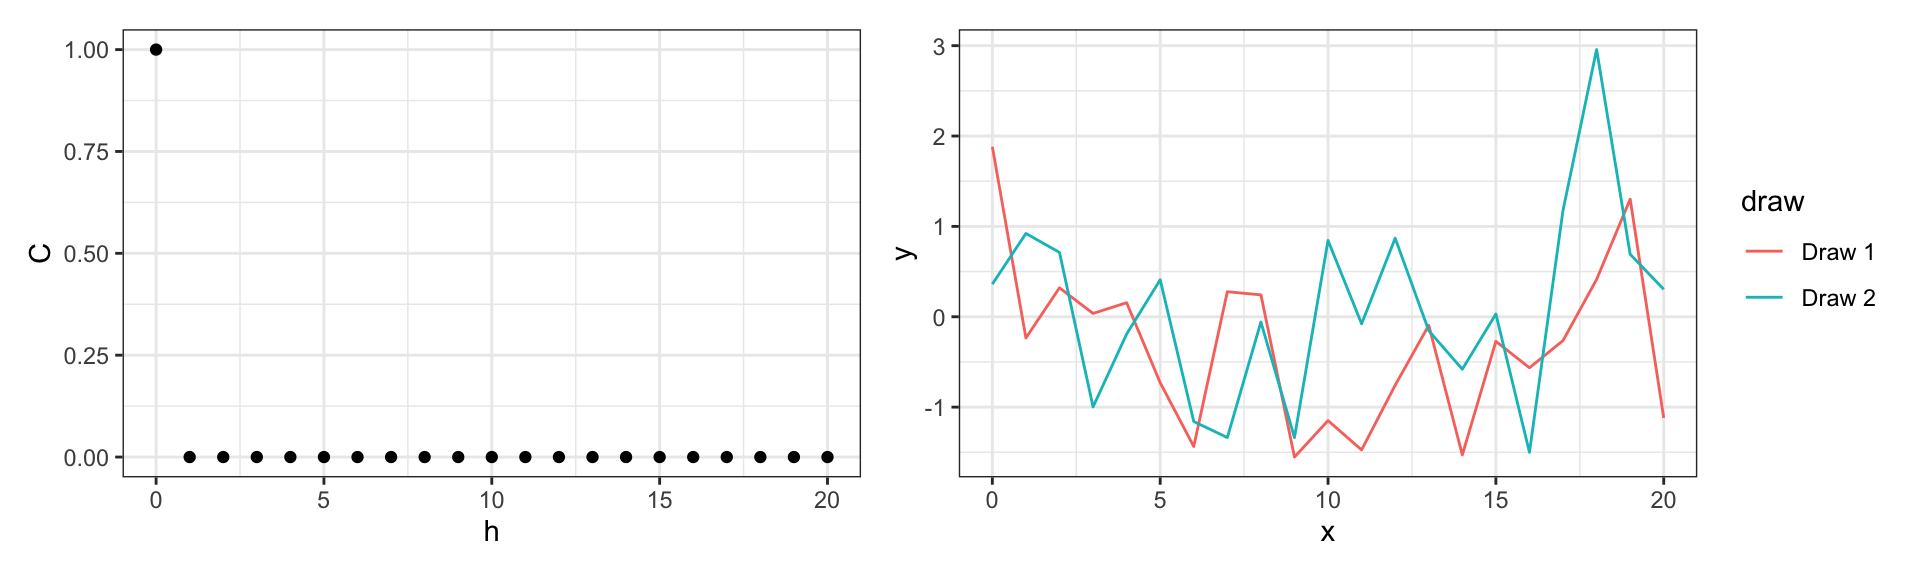
\includegraphics[width=\textwidth]{Lec21_files/figure-beamer/unnamed-chunk-1-1} \end{center}

\end{frame}

\begin{frame}{Practice - Migratory Model Prediction}
\protect\hypertarget{practice---migratory-model-prediction}{}

After fitting the GP need to sample from the posterior predictive
distribution at \(\sim3000\) locations
\[ \symbf{y}_{p} \sim \mathcal{N}\left(\mu_p + \Sigma_{po} \Sigma_o^{-1}(y_o - \mu_o) ,~ \Sigma_p - \Sigma_{po} \Sigma_{o}^{-1} \Sigma_{op}\right) \]

\pause

\scriptsize

\begin{longtable}[]{@{}ll@{}}
\toprule
\begin{minipage}[b]{0.59\columnwidth}\raggedright
Step\strut
\end{minipage} & \begin{minipage}[b]{0.35\columnwidth}\raggedright
CPU (secs)\strut
\end{minipage}\tabularnewline
\midrule
\endhead
\begin{minipage}[t]{0.59\columnwidth}\raggedright
1. Calc. \(\Sigma_p\), \(\Sigma_{po}\), \(\Sigma_{p}\)\strut
\end{minipage} & \begin{minipage}[t]{0.35\columnwidth}\raggedright
1.080\strut
\end{minipage}\tabularnewline
\begin{minipage}[t]{0.59\columnwidth}\raggedright
2. Calc.
\(\text{chol}(\Sigma_p - \Sigma_{po} \Sigma_{o}^{-1} \Sigma_{op})\)\strut
\end{minipage} & \begin{minipage}[t]{0.35\columnwidth}\raggedright
0.467\strut
\end{minipage}\tabularnewline
\begin{minipage}[t]{0.59\columnwidth}\raggedright
3. Calc. \(\mu_{p|o} + \text{chol}(\Sigma_{p|o}) \times Z\)\strut
\end{minipage} & \begin{minipage}[t]{0.35\columnwidth}\raggedright
0.049\strut
\end{minipage}\tabularnewline
\begin{minipage}[t]{0.59\columnwidth}\raggedright
4. Calc. Allele Prob\strut
\end{minipage} & \begin{minipage}[t]{0.35\columnwidth}\raggedright
0.129\strut
\end{minipage}\tabularnewline
\begin{minipage}[t]{0.59\columnwidth}\raggedright
Total\strut
\end{minipage} & \begin{minipage}[t]{0.35\columnwidth}\raggedright
1.732\strut
\end{minipage}\tabularnewline
\bottomrule
\end{longtable}

\normalsize

Total run time for 1000 posterior predictive draws:

\begin{itemize}
\tightlist
\item
  CPU (28.9 min)
\end{itemize}

\end{frame}

\begin{frame}{A bigger hammer?}
\protect\hypertarget{a-bigger-hammer}{}

\scriptsize

\begin{longtable}[]{@{}llll@{}}
\toprule
\begin{minipage}[b]{0.41\columnwidth}\raggedright
Step\strut
\end{minipage} & \begin{minipage}[b]{0.15\columnwidth}\raggedright
CPU (secs)\strut
\end{minipage} & \begin{minipage}[b]{0.19\columnwidth}\raggedright
CPU+GPU (secs)\strut
\end{minipage} & \begin{minipage}[b]{0.13\columnwidth}\raggedright
Rel. Perf\strut
\end{minipage}\tabularnewline
\midrule
\endhead
\begin{minipage}[t]{0.41\columnwidth}\raggedright
1. Calc. \(\Sigma_p\), \(\Sigma_{po}\), \(\Sigma_{p}\)\strut
\end{minipage} & \begin{minipage}[t]{0.15\columnwidth}\raggedright
1.080\strut
\end{minipage} & \begin{minipage}[t]{0.19\columnwidth}\raggedright
0.046\strut
\end{minipage} & \begin{minipage}[t]{0.13\columnwidth}\raggedright
23.0\strut
\end{minipage}\tabularnewline
\begin{minipage}[t]{0.41\columnwidth}\raggedright
2. Calc.
\(\text{chol}(\Sigma_p - \Sigma_{po} \Sigma_{o}^{-1} \Sigma_{op})\)\strut
\end{minipage} & \begin{minipage}[t]{0.15\columnwidth}\raggedright
0.467\strut
\end{minipage} & \begin{minipage}[t]{0.19\columnwidth}\raggedright
0.208\strut
\end{minipage} & \begin{minipage}[t]{0.13\columnwidth}\raggedright
2.3\strut
\end{minipage}\tabularnewline
\begin{minipage}[t]{0.41\columnwidth}\raggedright
3. Calc. \(\mu_{p|o} + \text{chol}(\Sigma_{p|o}) \times Z\)\strut
\end{minipage} & \begin{minipage}[t]{0.15\columnwidth}\raggedright
0.049\strut
\end{minipage} & \begin{minipage}[t]{0.19\columnwidth}\raggedright
0.052\strut
\end{minipage} & \begin{minipage}[t]{0.13\columnwidth}\raggedright
0.9\strut
\end{minipage}\tabularnewline
\begin{minipage}[t]{0.41\columnwidth}\raggedright
4. Calc. Allele Prob\strut
\end{minipage} & \begin{minipage}[t]{0.15\columnwidth}\raggedright
0.129\strut
\end{minipage} & \begin{minipage}[t]{0.19\columnwidth}\raggedright
0.127\strut
\end{minipage} & \begin{minipage}[t]{0.13\columnwidth}\raggedright
1.0\strut
\end{minipage}\tabularnewline
\begin{minipage}[t]{0.41\columnwidth}\raggedright
Total\strut
\end{minipage} & \begin{minipage}[t]{0.15\columnwidth}\raggedright
1.732\strut
\end{minipage} & \begin{minipage}[t]{0.19\columnwidth}\raggedright
0.465\strut
\end{minipage} & \begin{minipage}[t]{0.13\columnwidth}\raggedright
3.7\strut
\end{minipage}\tabularnewline
\bottomrule
\end{longtable}

\normalsize

Total run time for 1000 posterior predictive draws:

\begin{itemize}
\tightlist
\item
  CPU (28.9 min)
\item
  CPU+GPU (7.8 min)
\end{itemize}

\end{frame}

\begin{frame}{Cholesky CPU vs GPU (P100)}
\protect\hypertarget{cholesky-cpu-vs-gpu-p100}{}

\begin{center}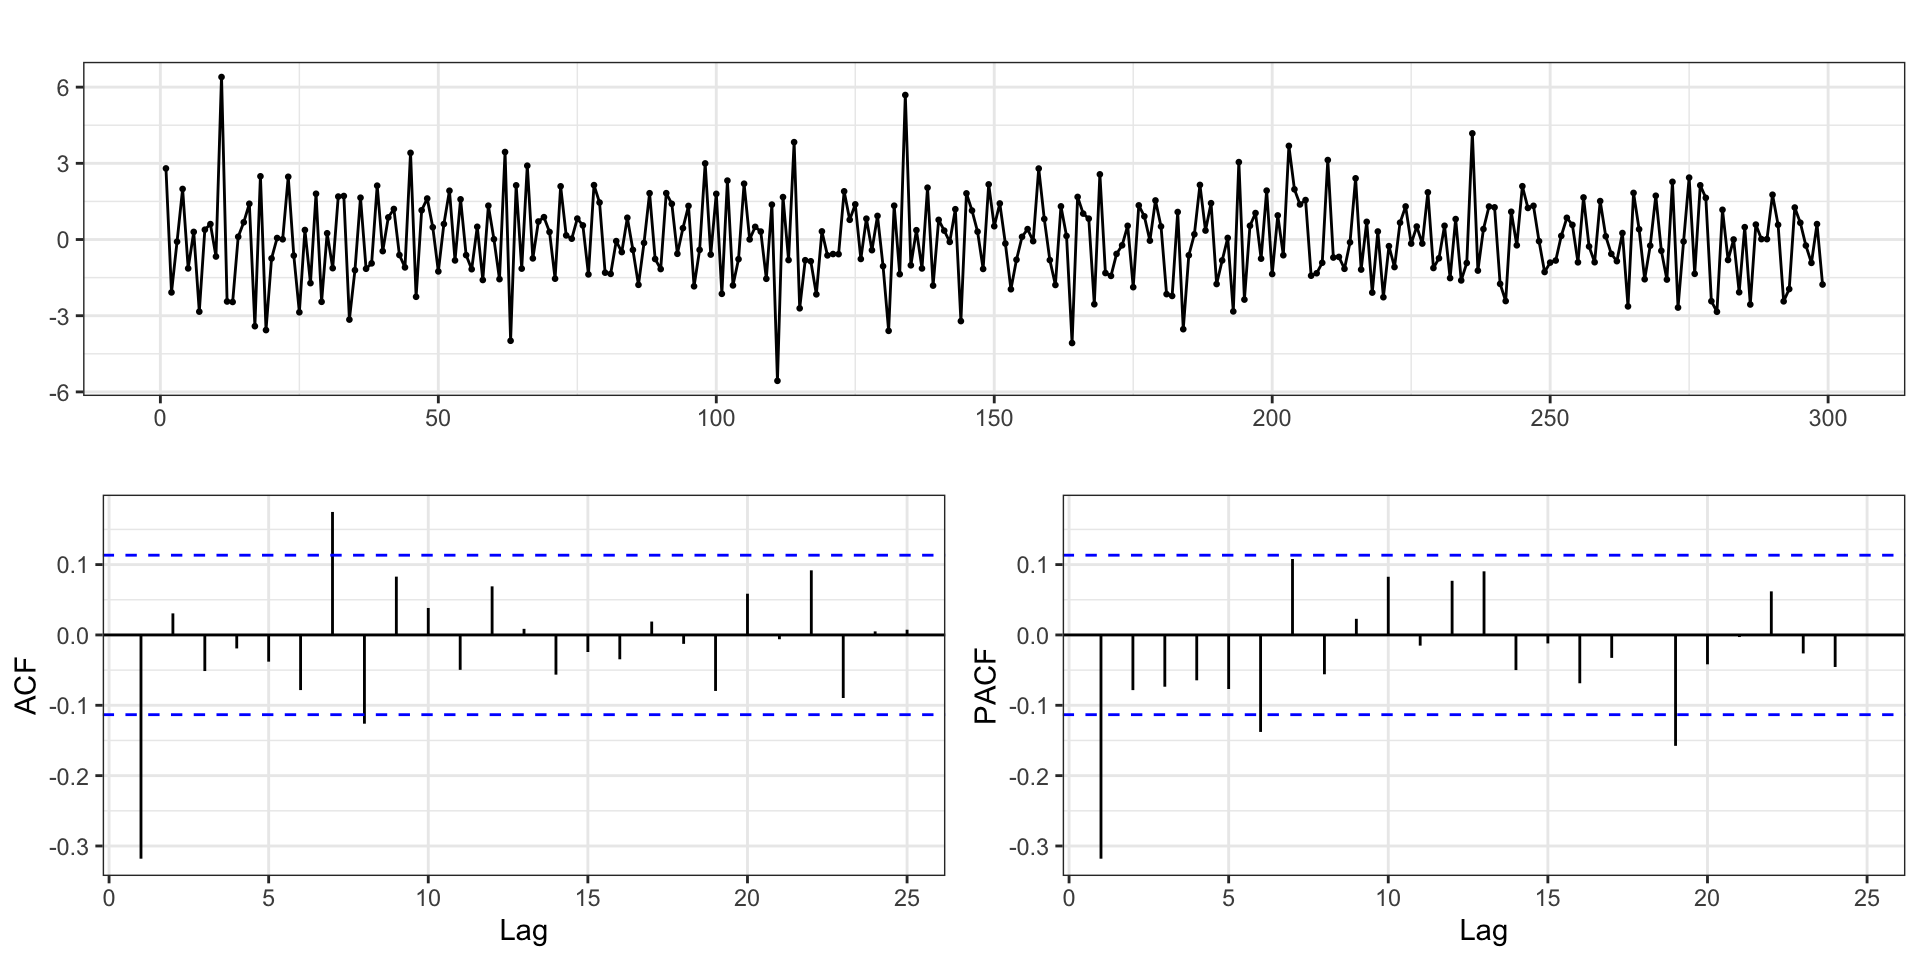
\includegraphics[width=\textwidth]{Lec21_files/figure-beamer/unnamed-chunk-2-1} \end{center}

\end{frame}

\begin{frame}{}
\protect\hypertarget{section}{}

\begin{center}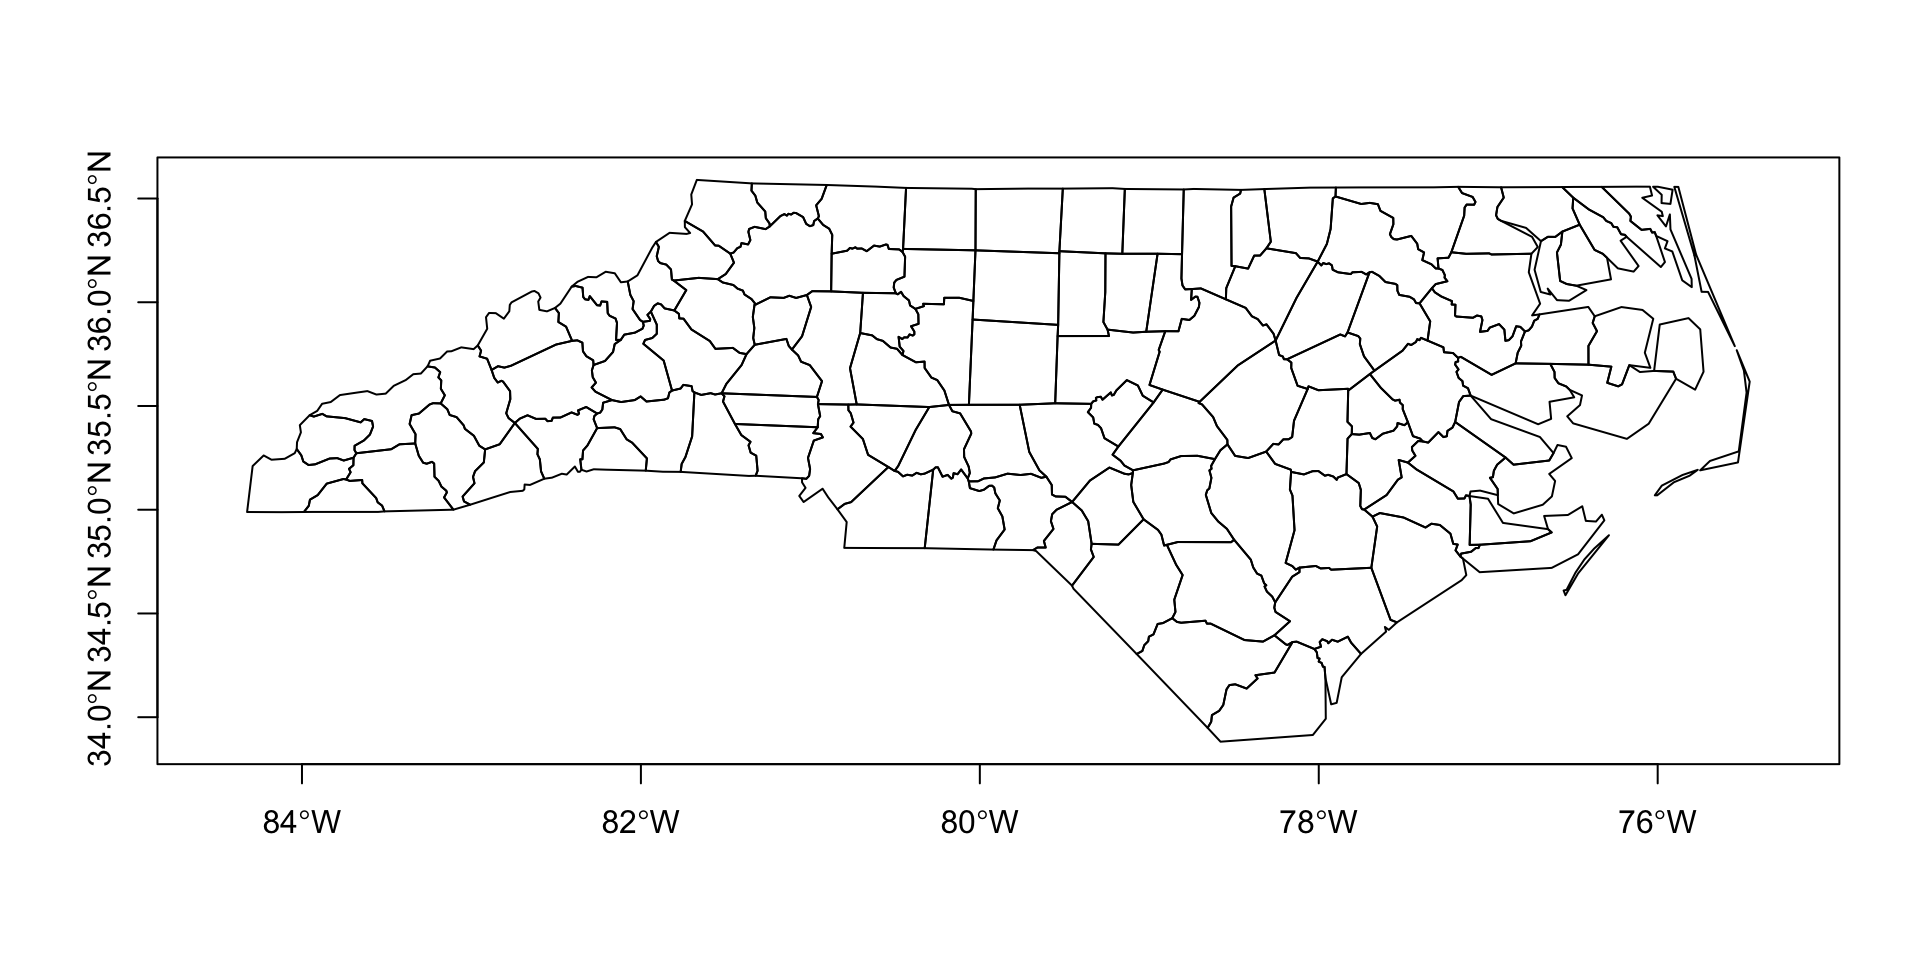
\includegraphics[width=\textwidth]{Lec21_files/figure-beamer/unnamed-chunk-3-1} \end{center}

\end{frame}

\begin{frame}{Relative Performance}
\protect\hypertarget{relative-performance}{}

\begin{center}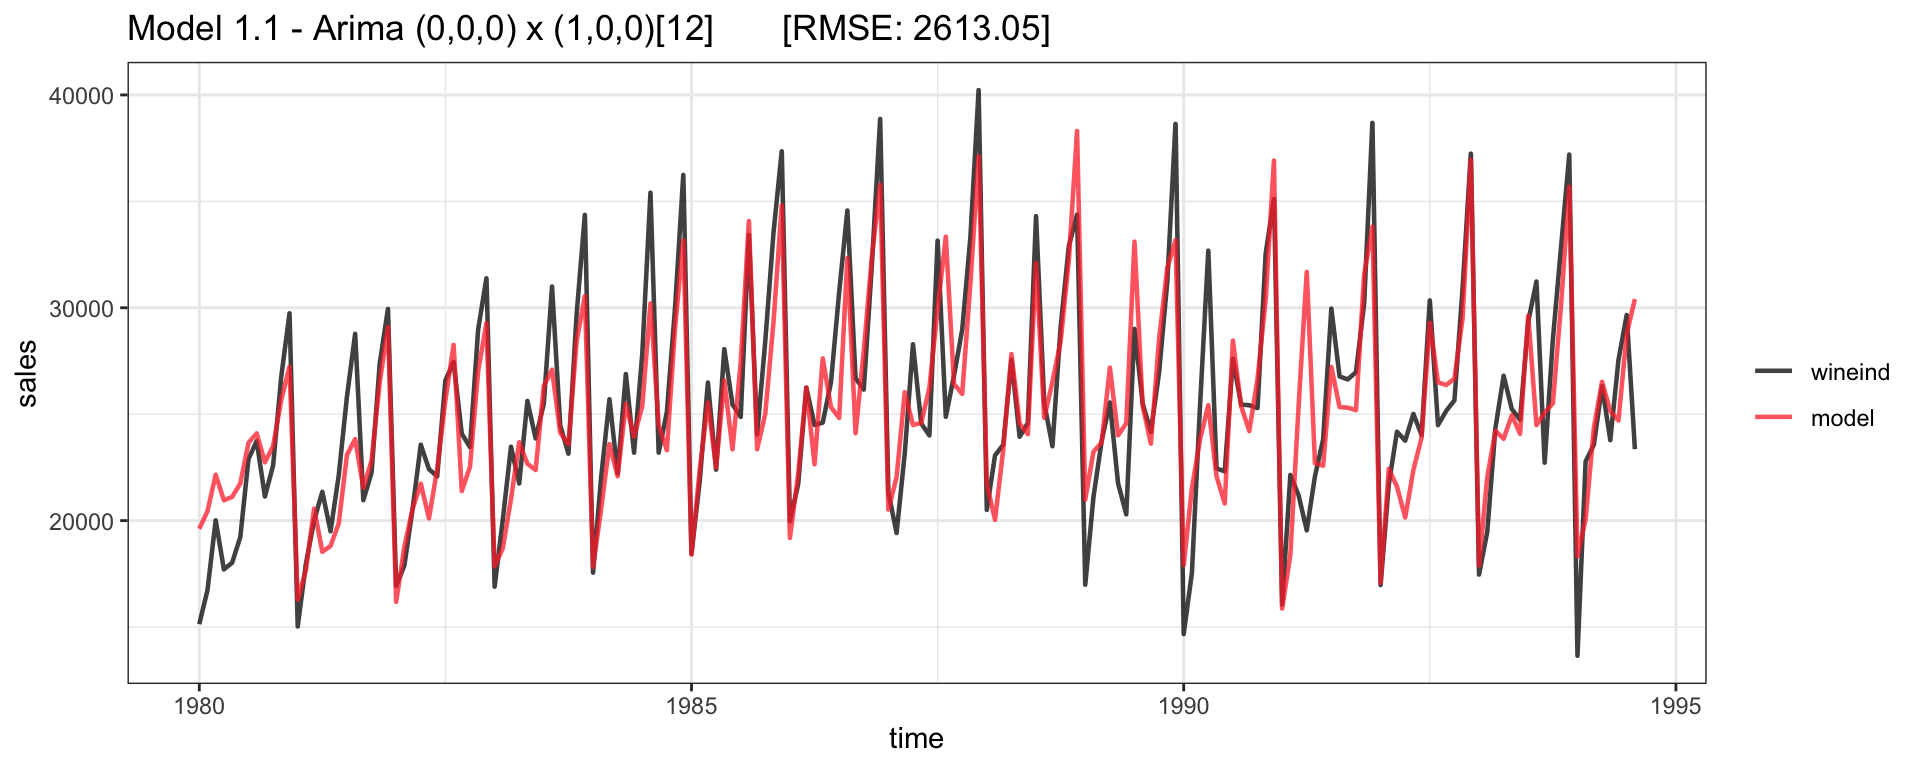
\includegraphics[width=\textwidth]{Lec21_files/figure-beamer/unnamed-chunk-4-1} \end{center}

\end{frame}

\begin{frame}{Aside (1) - Matrix Multiplication}
\protect\hypertarget{aside-1---matrix-multiplication}{}

\begin{center}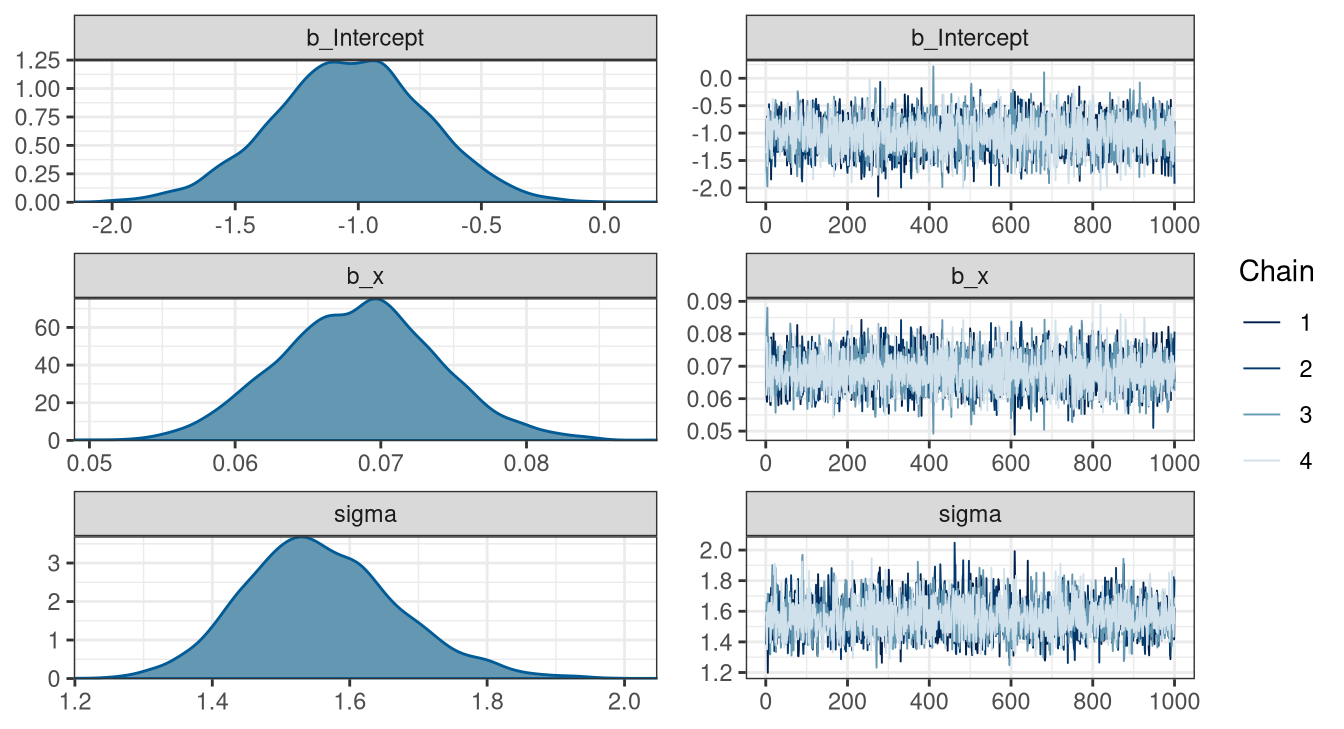
\includegraphics[width=\textwidth]{Lec21_files/figure-beamer/unnamed-chunk-5-1} \end{center}

\end{frame}

\begin{frame}{}
\protect\hypertarget{section-1}{}

\begin{center}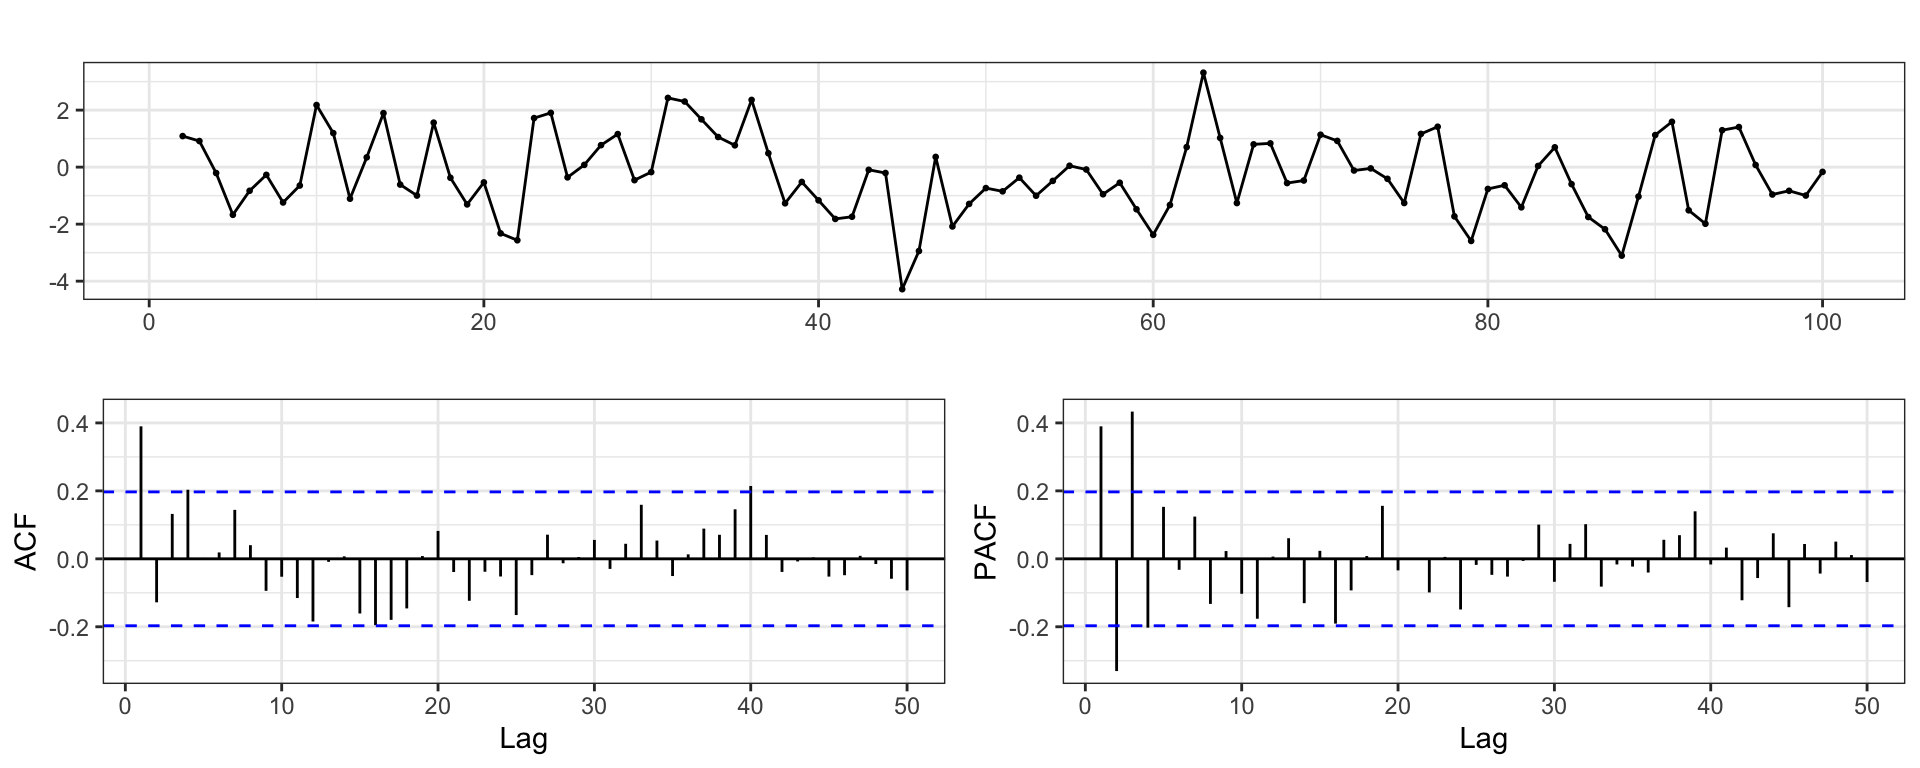
\includegraphics[width=\textwidth]{Lec21_files/figure-beamer/unnamed-chunk-6-1} \end{center}

\end{frame}

\begin{frame}{Aside (2) - Memory Limitations}
\protect\hypertarget{aside-2---memory-limitations}{}

A general covariance is a dense \(n \times n\) matrix, meaning it will
require \(n^2 \times\) 64-bits to store.

\begin{center}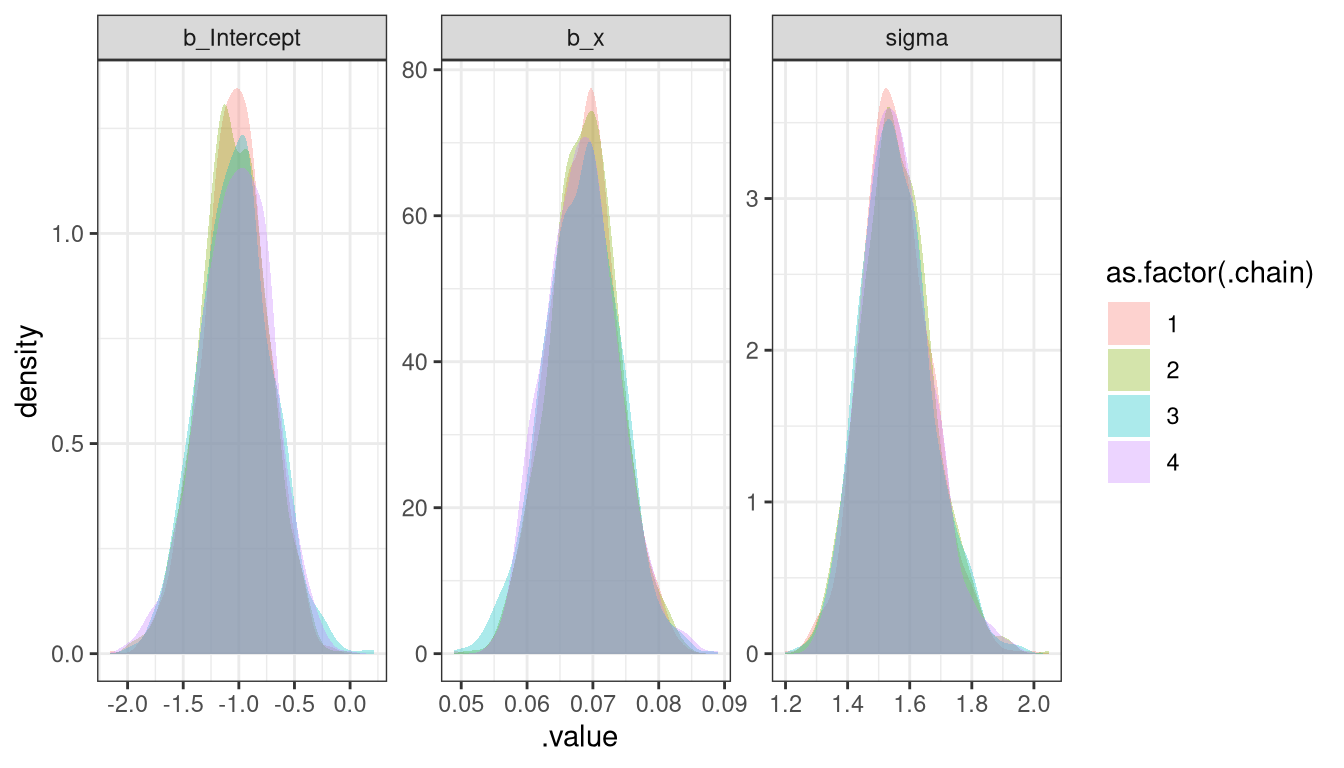
\includegraphics[width=\textwidth]{Lec21_files/figure-beamer/unnamed-chunk-7-1} \end{center}

\end{frame}

\begin{frame}[fragile]{Other big hammers}
\protect\hypertarget{other-big-hammers}{}

\small

\texttt{bigGP} is an R package written by Chris Paciorek (UC Berkeley),
et al.

\begin{itemize}
\item
  Specialized distributed implementation of linear algebra operation for
  GPs
\item
  Designed to run on large super computer clusters
\item
  Uses both shared and distributed memory
\item
  Able to fit models on the order of \(n = 65\)k (32 GB Cov. matrix)
\end{itemize}

\vspace{-3mm}

\begin{center}
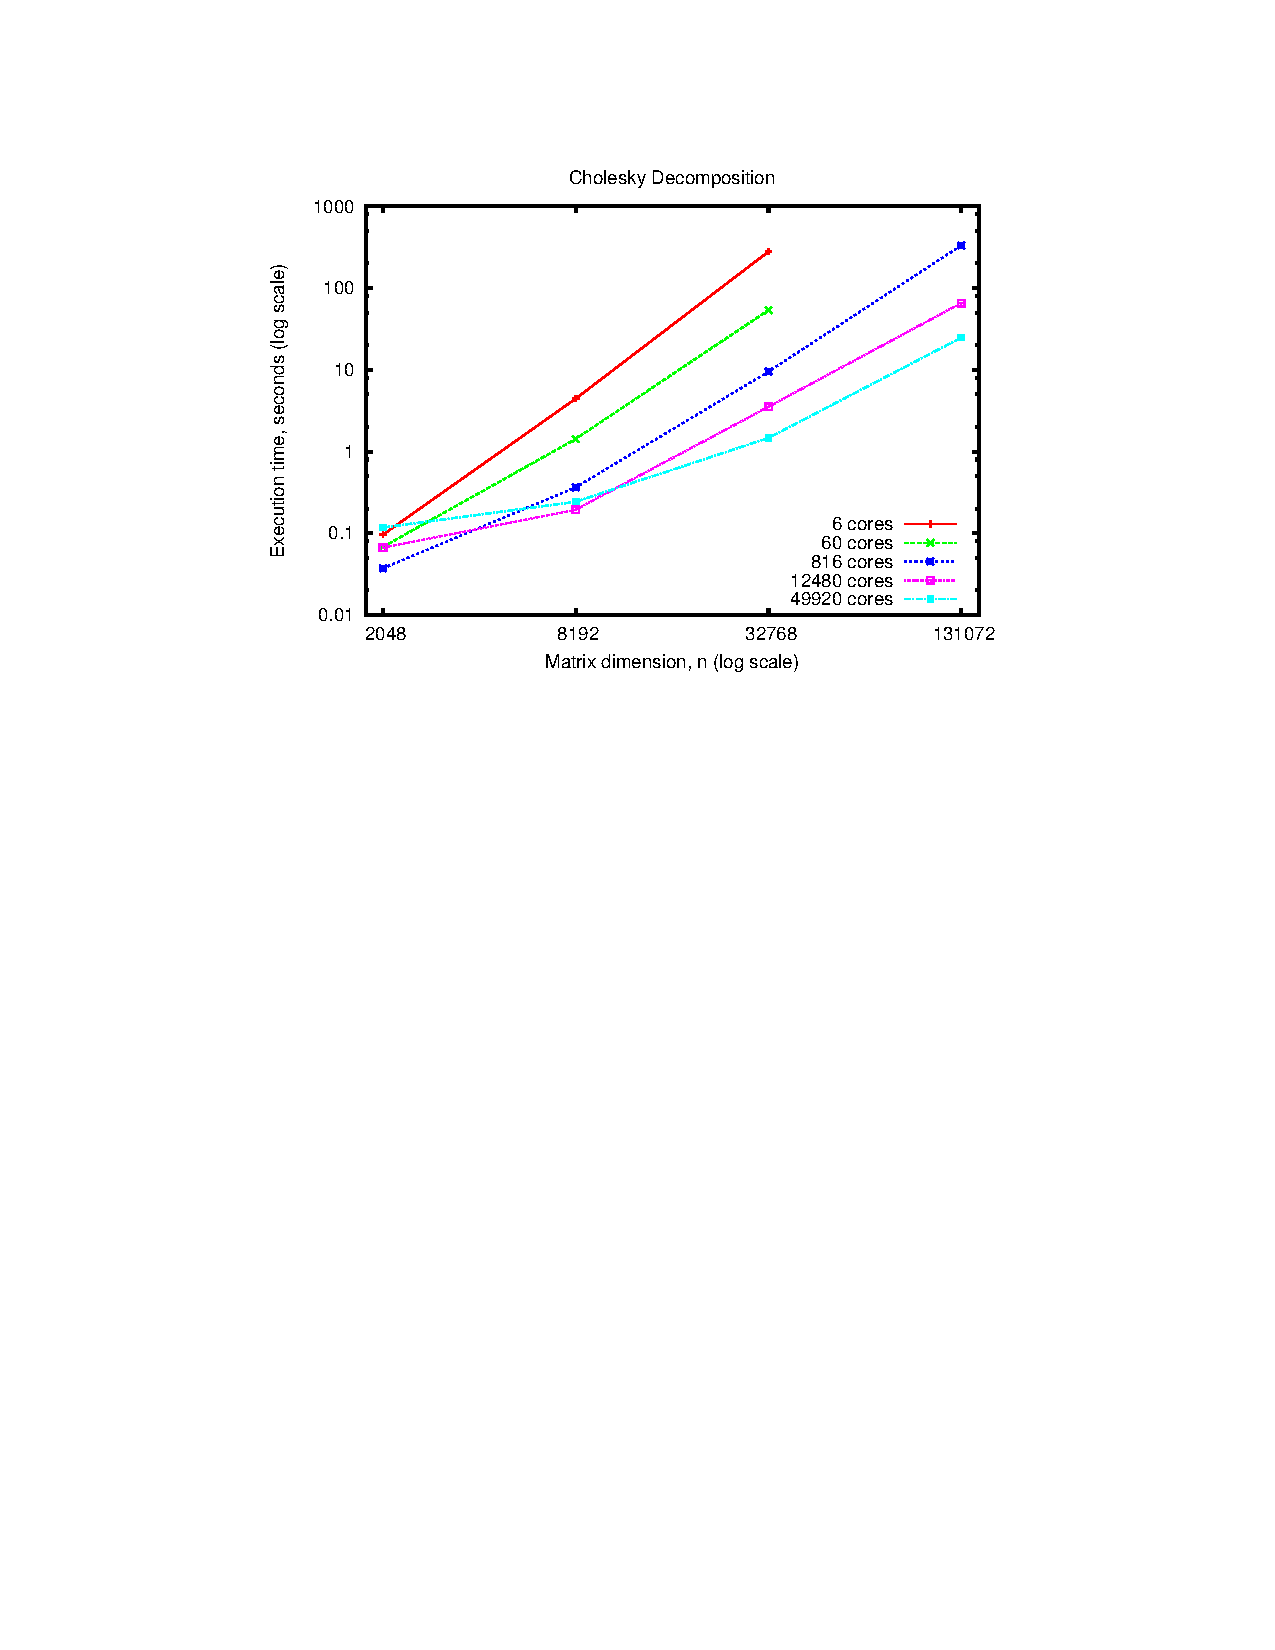
\includegraphics[width=0.7\textwidth]{figs/Paciorek.pdf}
\end{center}

\end{frame}

\begin{frame}{More scalable solutions?}
\protect\hypertarget{more-scalable-solutions}{}

\large

\begin{itemize}
\tightlist
\item
  Spectral domain / basis functions
\end{itemize}

\vspace{3mm}

\begin{itemize}
\tightlist
\item
  Covariance tapering
\end{itemize}

\vspace{3mm}

\begin{itemize}
\tightlist
\item
  GMRF approximations
\end{itemize}

\vspace{3mm}

\begin{itemize}
\tightlist
\item
  Low-rank approximations
\end{itemize}

\vspace{3mm}

\begin{itemize}
\tightlist
\item
  Nearest-neighbor models
\end{itemize}

\end{frame}

\hypertarget{low-rank-approximations}{%
\section{Low Rank Approximations}\label{low-rank-approximations}}

\begin{frame}{Low rank approximations in general}
\protect\hypertarget{low-rank-approximations-in-general}{}

Lets look at the example of the singular value decomposition of a
matrix,

\[ \underset{n \times m}{M} = \underset{n \times n}{U}\,\underset{n \times m}{\text{diag}(S)}\,\underset{m \times m}{V^{\,t}} \]
where \(U\) are called the left singular vectors, \(V\) the right
singular vectors, and \(S\) the singular values. Usually the singular
values and vectors are ordered such that the singular values are in
descending order.

\pause

The Eckart--Young theorem states that we can construct an
approximatation of \(M\) with rank \(k\) by setting \(\tilde S\) to
contain only the \(k\) largest singular values and all other values set
to zero.

\[ 
\begin{aligned}
\underset{n \times m}{\tilde M} 
  &= \underset{n \times n}{U}\,\underset{n \times m}{\text{diag}(\tilde S)}\,\underset{m \times m}{V^{\,t}} \\
  &= \underset{n \times k}{\tilde U}\,\underset{k \times k}{\text{diag}(\tilde S)}\,\underset{k \times m}{\tilde{V}^{\,t}} 
\end{aligned}
\]

\end{frame}

\begin{frame}{Example}
\protect\hypertarget{example}{}

\footnotesize

\[ \begin{aligned}
M 
&= \begin{pmatrix}
  1.000 & 0.500 & 0.333 & 0.250 \\ 
  0.500 & 0.333 & 0.250 & 0.200 \\ 
  0.333 & 0.250 & 0.200 & 0.167 \\ 
  0.250 & 0.200 & 0.167 & 0.143 \\ 
\end{pmatrix} 
  = U \, \text{diag}(S) \, V^{\,t} \\
U = V &= \begin{pmatrix}
  -0.79 & 0.58 & -0.18 & -0.03 \\ 
  -0.45 & -0.37 & 0.74 & 0.33 \\ 
  -0.32 & -0.51 & -0.10 & -0.79 \\ 
  -0.25 & -0.51 & -0.64 & 0.51 \\ 
  \end{pmatrix} \\
S &= 
\begin{pmatrix} 1.50 & 0.17  & 0.01 & 0.00 \end{pmatrix}
\end{aligned} \]

\pause

\normalsize

Rank 2 approximation: \footnotesize \[ \begin{aligned}
\tilde M
&= \begin{pmatrix}
  -0.79 &  0.58 \\ 
  -0.45 & -0.37 \\ 
  -0.32 & -0.51 \\ 
  -0.25 & -0.51 \\ 
\end{pmatrix}
\begin{pmatrix}
  1.50 & 0.00 \\ 
  0.00 & 0.17 \\ 
\end{pmatrix}
\begin{pmatrix}
  -0.79 & -0.45 & -0.32 & -0.25 \\ 
  0.58 & -0.37 & -0.51 & -0.51 \\ 
\end{pmatrix} \\
&= 
\begin{pmatrix}
  1.000 & 0.501 & 0.333 & 0.249 \\ 
  0.501 & 0.330 & 0.251 & 0.203 \\ 
  0.333 & 0.251 & 0.200 & 0.166 \\ 
  0.249 & 0.203 & 0.166 & 0.140 \\ 
\end{pmatrix}
\end{aligned} \]

\end{frame}

\begin{frame}{Approximation Error}
\protect\hypertarget{approximation-error}{}

We can measure the error of the approximation using the Frobenius norm,
\[ \lVert M-\tilde M\rVert_F = \left( \sum_{i=1}^m\sum_{j=1}^n (M_{ij}-\tilde M_{ij})^2\right)^{1/2} \]

\pause

\[  M-\tilde M = 
\begin{pmatrix}
  0.00022 & -0.00090 & 0.00012 & 0.00077 \\ 
  -0.00090 & 0.00372 & -0.00053 & -0.00317 \\ 
  0.00012 & -0.00053 & 0.00013 & 0.00039 \\ 
  0.00077 & -0.00317 & 0.00039 & 0.00277 \\ 
\end{pmatrix}
\]

\[ \lVert M-\tilde M\rVert_F = 0.00674 \]

\end{frame}

\begin{frame}{Cov Mat - Strong dependence (large eff. range):}
\protect\hypertarget{cov-mat---strong-dependence-large-eff.-range}{}

\begin{center}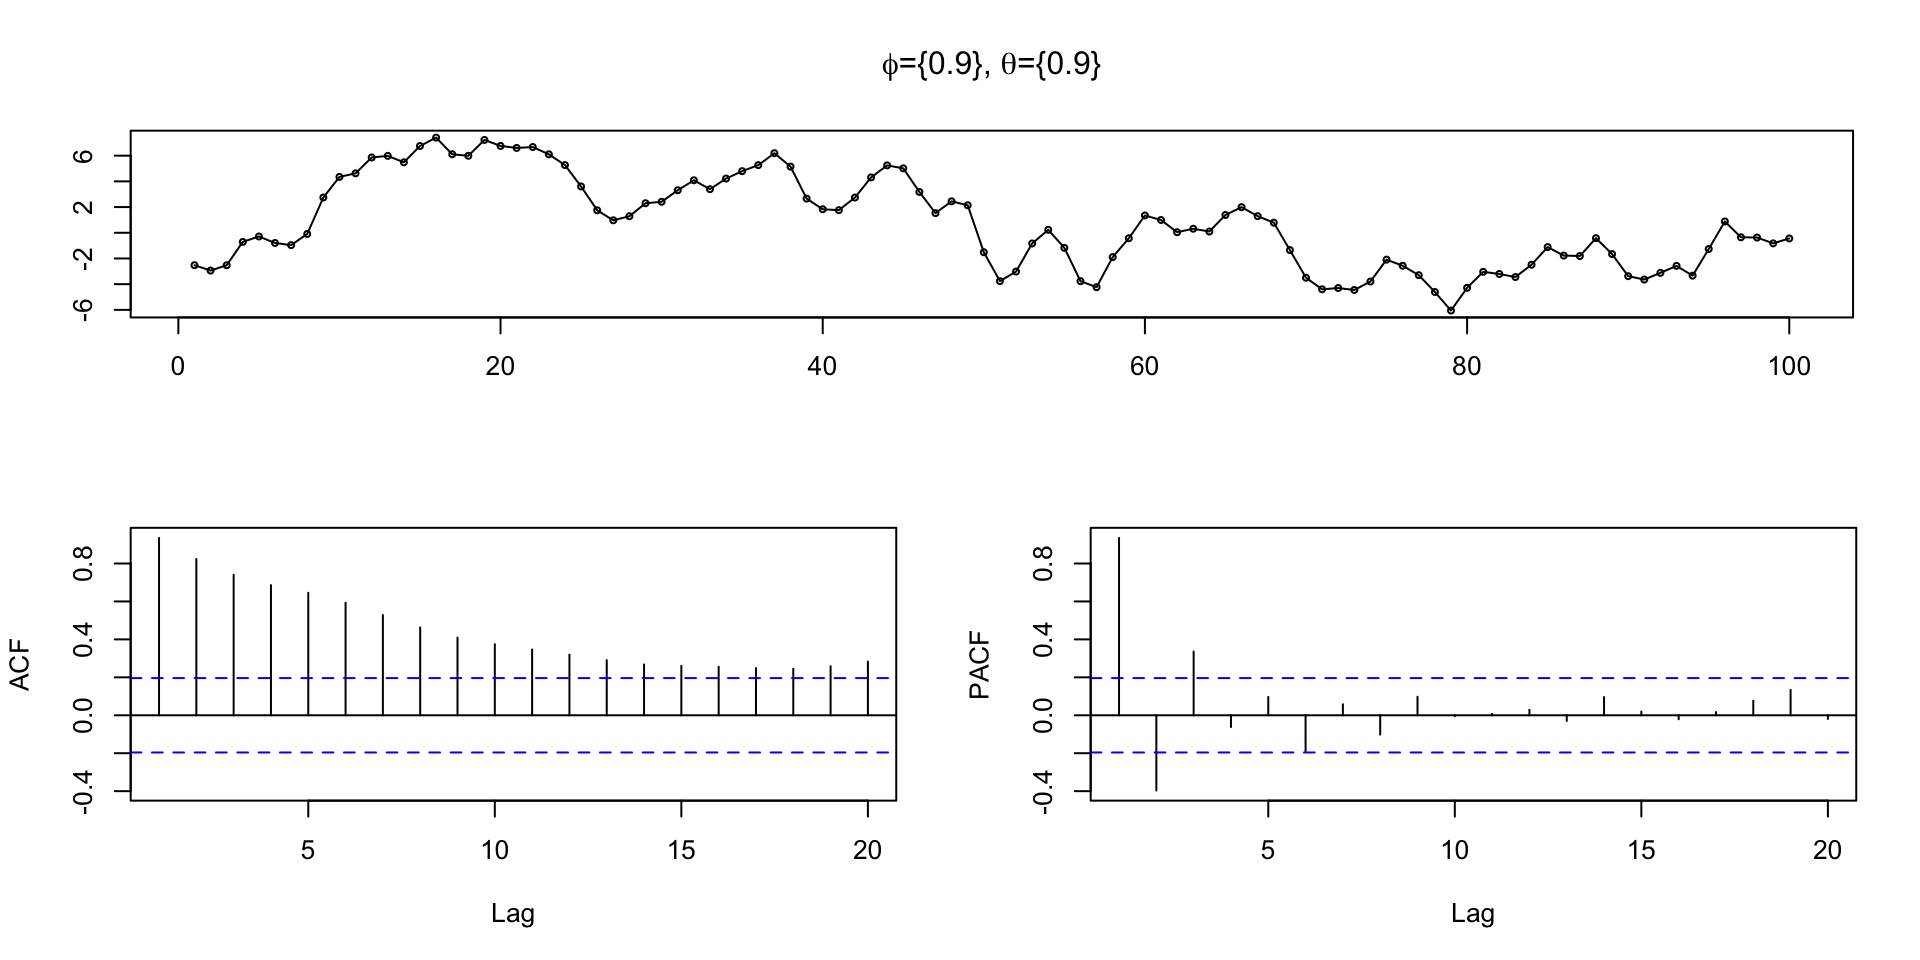
\includegraphics[width=\textwidth]{Lec21_files/figure-beamer/unnamed-chunk-9-1} \end{center}

\end{frame}

\begin{frame}{Cov Mat - Weak dependence (short eff. range):}
\protect\hypertarget{cov-mat---weak-dependence-short-eff.-range}{}

\begin{center}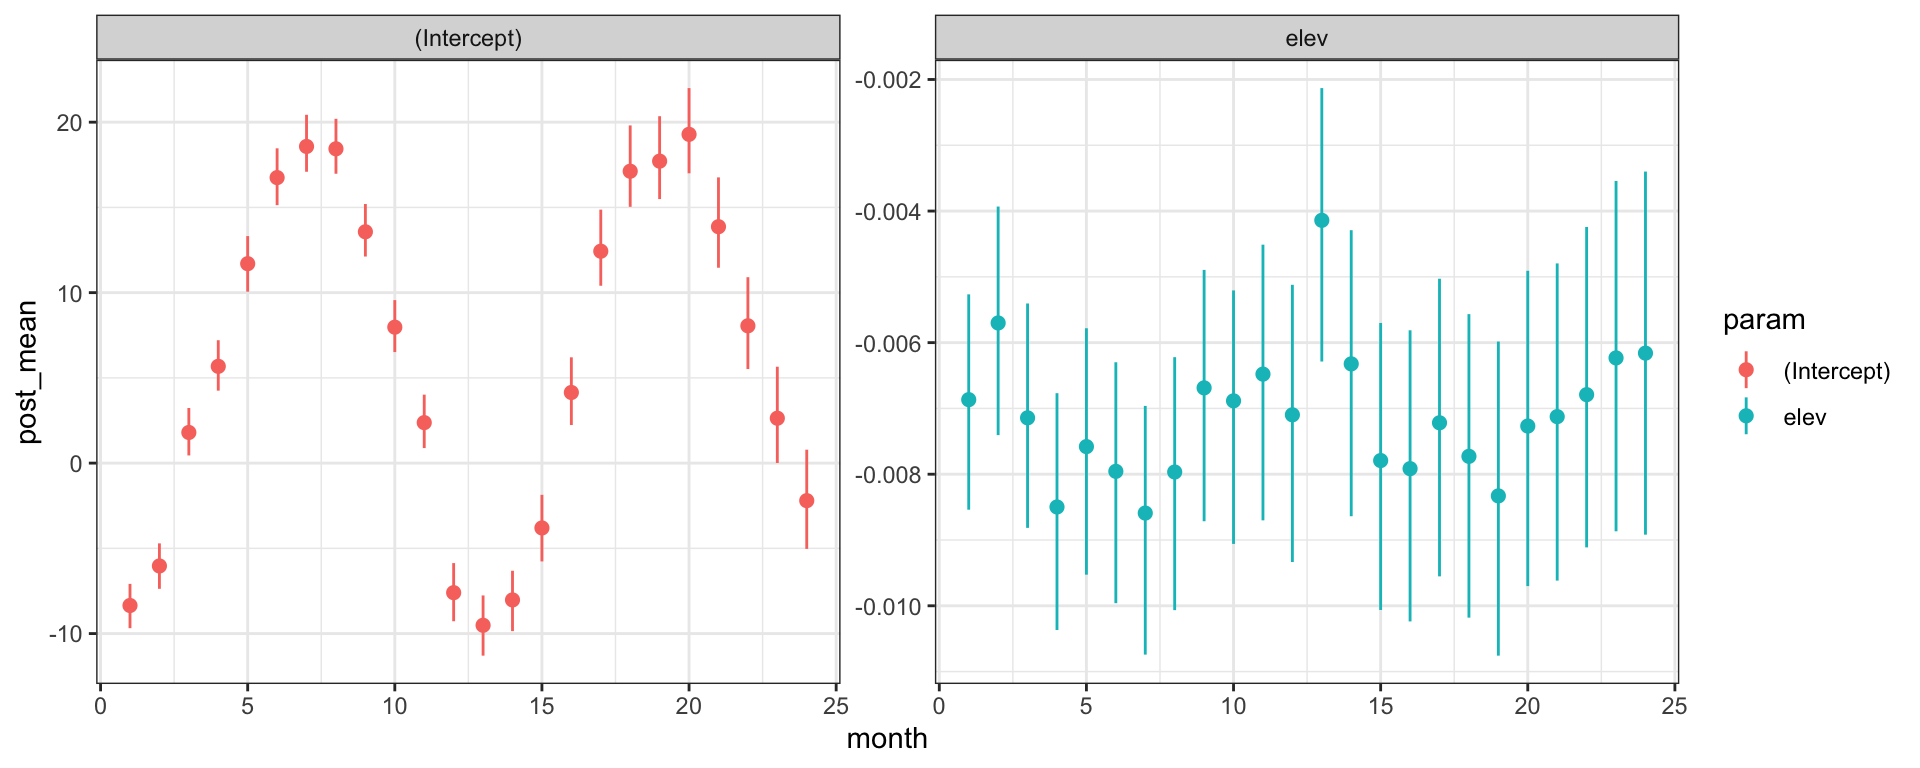
\includegraphics[width=\textwidth]{Lec21_files/figure-beamer/unnamed-chunk-10-1} \end{center}

\end{frame}

\begin{frame}[t]{How does this help? (Sherman-Morrison-Woodbury)}
\protect\hypertarget{how-does-this-help-sherman-morrison-woodbury}{}

There is an immensely useful linear algebra identity, the
Sherman-Morrison-\emph{Woodbury} formula, for the inverse (and
determinant) of a decomposed matrix,

\[\begin{aligned}
\underset{n \times m}{M}^{-1} 
&= \left(\underset{n \times m}{A} + \underset{n \times k}{U} ~ \underset{k \times k}{S} ~ \underset{k \times m}{V^t}\right)^{-1} \\
&= A^{-1} - A^{-1} U \left(S^{-1}+V^{\,t} A^{-1} U\right)^{-1}V^{\,t} A^{-1}.
\end{aligned}\]

\pause

How does this help?

\begin{itemize}
\item
  Imagine that \(A = \text{diag}(A)\), then it is trivial to find
  \(A^{-1}\).
\item
  \(S^{-1}\) is \(k \times k\) which is hopefully small, or even better
  \(S = \text{diag}(S)\).
\item
  \(\left(S^{-1}+V^{\,t} A^{-1} U\right)\) is \(k \times k\) which is
  also small.
\end{itemize}

\end{frame}

\begin{frame}{Aside - Determinant}
\protect\hypertarget{aside---determinant}{}

Remember for any MVN distribution when evaluating the likelihood
\[ -\frac{1}{2} \log {|\Sigma|} - \frac{1}{2} (\symbf{x}-\symbf{\mu})' {\symbf{\Sigma}^{-1}} (\symbf{x}-\symbf{\mu}) - \frac{n}{2}\log 2\pi\]
we need the inverse of \(\Sigma\) as well as its \emph{determinant}.

\pause

\begin{itemize}
\tightlist
\item
  For a full rank Cholesky decomposition we get the determinant for
  ``free''.
\end{itemize}

\vspace{-3mm}

\[|M| = |LL^t| = \prod_{i=1}^n \left(\text{diag}(L)_i\right)^2\]

\pause

\begin{itemize}
\tightlist
\item
  The Sherman-Morrison-Woodbury Determinant lemma gives us,
\end{itemize}

\vspace{-3mm}

\[\begin{aligned}
\det(M) 
  &= \det({A} + {U} {S} {V^t}) \\
  &= \det(S^{-1} + V^t A^{-1} U) ~ \det(S) ~ \det(A)
\end{aligned}\]

\end{frame}

\begin{frame}[t]{Low rank approximations for GPs}
\protect\hypertarget{low-rank-approximations-for-gps}{}

For a standard spatial random effects model,

\[ y(\symbf{s}) = x(\symbf{s}) \, \symbf{\beta} + w(\symbf{s}) + \epsilon, \quad \epsilon \sim N(0,~\tau^2 I) \]
\[ w(\symbf{s}) \sim \mathcal{N}(0,~\symbf{\Sigma}(\symbf{s})), \quad \symbf{\Sigma}(\symbf{s},\symbf{s}')=\sigma\,\rho(\symbf{s},\symbf{s}'|\theta) \]

if we can replace \(\symbf{\Sigma}(\symbf{s})\) with a low rank
approximation of the form

\begin{itemize}
\item
  \(\symbf{\Sigma}(\symbf{s}) \approx \symbf{U}\,\symbf{S}\,\symbf{V}^t\)
  where
\item
  \(\symbf{U}\) and \(\symbf{V}\) are \(n \times k\),
\item
  \(\symbf{S}\) is \(k \times k\), and
\item
  \(A = \tau^2 I\) or a similar diagonal matrix
\end{itemize}

\end{frame}

\hypertarget{predictive-processes}{%
\section{Predictive Processes}\label{predictive-processes}}

\begin{frame}{Gaussian Predictive Processes}
\protect\hypertarget{gaussian-predictive-processes}{}

\small

For a rank \(k\) approximation,

\begin{itemize}
\tightlist
\item
  Pick \(k\) knot locations \(\symbf{s}^\star\)
\end{itemize}

\pause

\begin{itemize}
\tightlist
\item
  Calculate knot covariance, \(\symbf{\Sigma}(\symbf{s}^\star)\), and
  knot cross-covariance, \(\symbf{\Sigma}(\symbf{s}, \symbf{s}^\star)\)
\end{itemize}

\pause

\begin{itemize}
\tightlist
\item
  Approximate full covariance using
\end{itemize}

\vspace{-2mm}

\[ \symbf{\Sigma}(\symbf{s}) \approx \underset{n \times k}{\symbf{\Sigma}(\symbf{s},\symbf{s}^\star)} \, \underset{k \times k}{\symbf{\Sigma}(\symbf{s}^\star)^{-1}} \, \underset{k \times n}{\symbf{\Sigma}(\symbf{s}^\star,\symbf{s})}. \]

\pause

\begin{itemize}
\tightlist
\item
  PPs systematically underestimates variance (\(\sigma^2\)) and inflate
  \(\tau^2\), Modified predictive processs corrects this using
\end{itemize}

\vspace{-2mm}

\[
\begin{aligned}
\symbf{\Sigma}(\symbf{s}) \approx &
\symbf{\Sigma}(\symbf{s},\symbf{s}^\star) \, \symbf{\Sigma}(\symbf{s}^\star)^{-1} \, \symbf{\Sigma}(\symbf{s}^\star,\symbf{s}) \\
&+ \text{diag}\Big(\symbf{\Sigma}(\symbf{s}) - \symbf{\Sigma}(\symbf{s},\symbf{s}^\star) \, \symbf{\Sigma}(\symbf{s}^\star)^{-1} \, \symbf{\Sigma}(\symbf{s}^\star,\symbf{s})\Big).
\end{aligned}
\]

\vspace{4mm}

\footnotesize
\begin{center}
Banerjee, Gelfand, Finley, Sang (2008) \quad Finley, Sang, Banerjee, Gelfand (2008)
\end{center}

\end{frame}

\begin{frame}{Example}
\protect\hypertarget{example-1}{}

Below we have a surface generate from a squared exponential Gaussian
Process where
\[ \{\Sigma\}_{ij} = \sigma^2 \exp\left(-(\phi\,d)^2\right) + \tau^2 I \]
\[ \sigma^2 = 1 \quad \phi=9 \quad \tau^2 = 0.1 \]

\begin{center}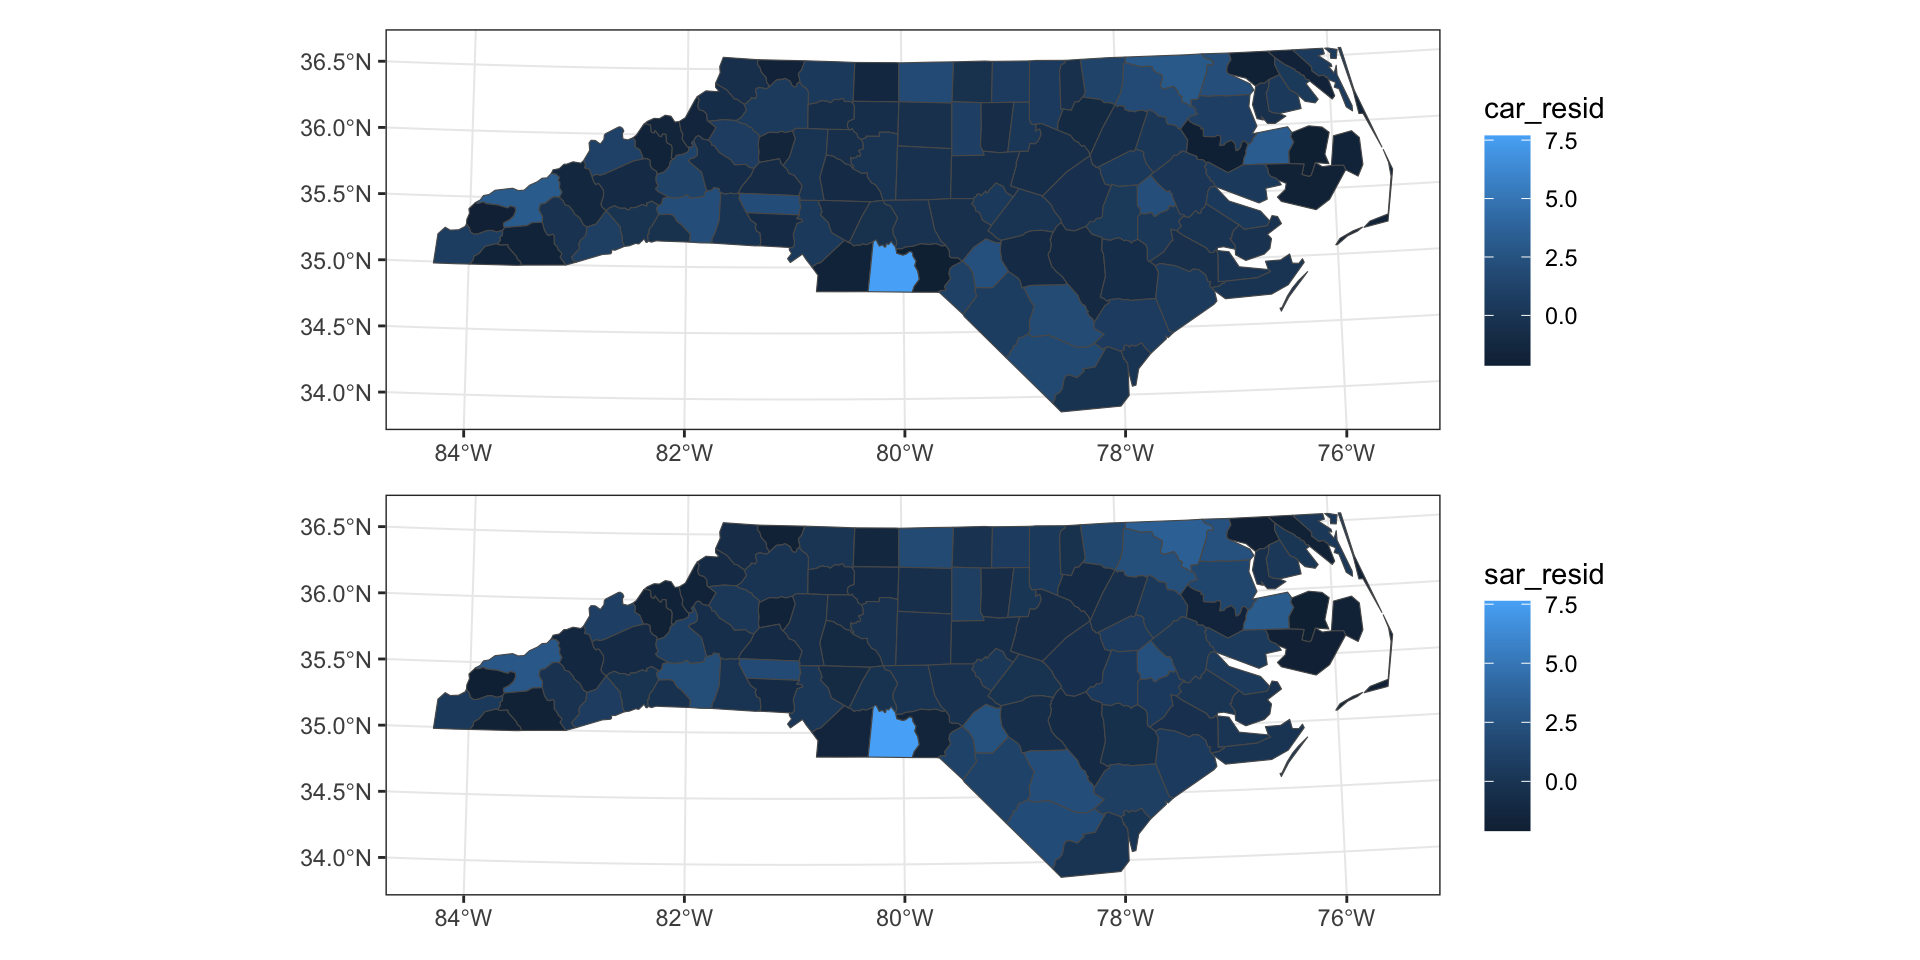
\includegraphics[width=\textwidth]{Lec21_files/figure-beamer/unnamed-chunk-12-1} \end{center}

\end{frame}

\begin{frame}{Predictive Process Model Results}
\protect\hypertarget{predictive-process-model-results}{}

\begin{center}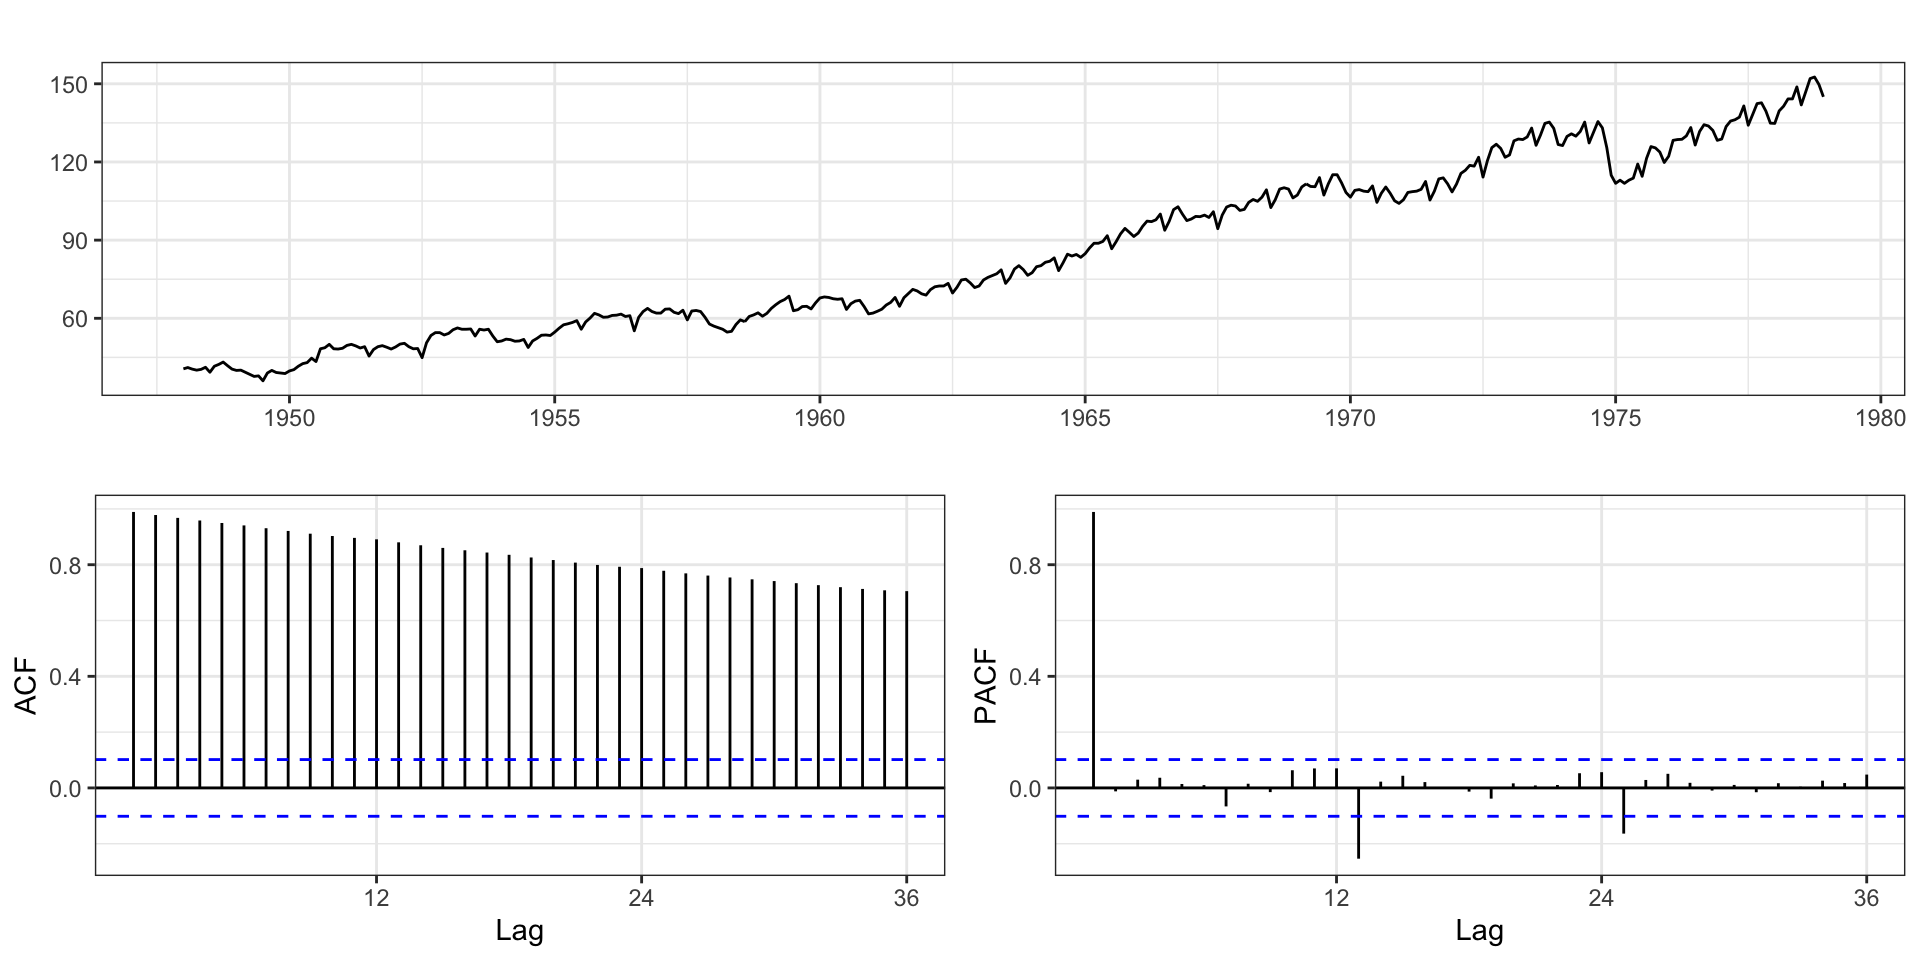
\includegraphics[width=\textwidth]{Lec21_files/figure-beamer/unnamed-chunk-15-1} \end{center}

\end{frame}

\begin{frame}{Performance}
\protect\hypertarget{performance}{}

\begin{center}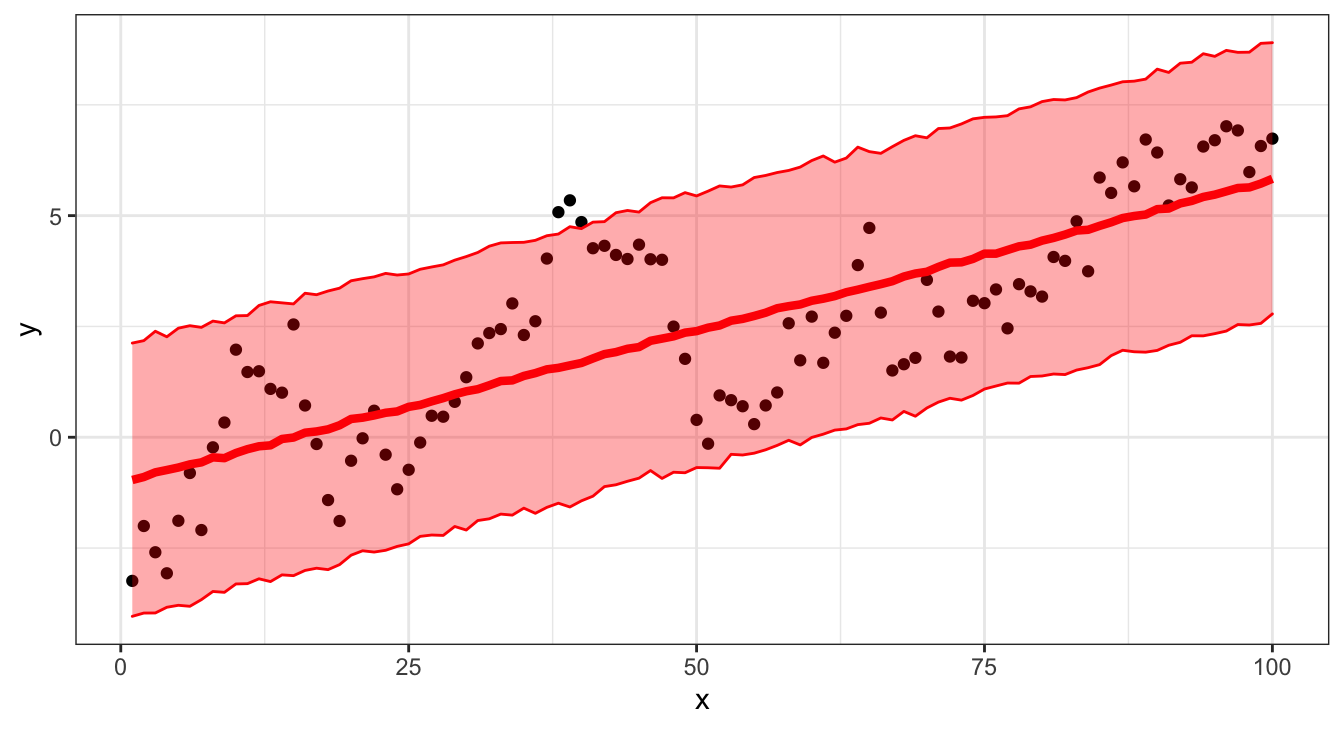
\includegraphics[width=\textwidth]{Lec21_files/figure-beamer/unnamed-chunk-16-1} \end{center}

\end{frame}

\begin{frame}{Parameter Estimates}
\protect\hypertarget{parameter-estimates}{}

\begin{center}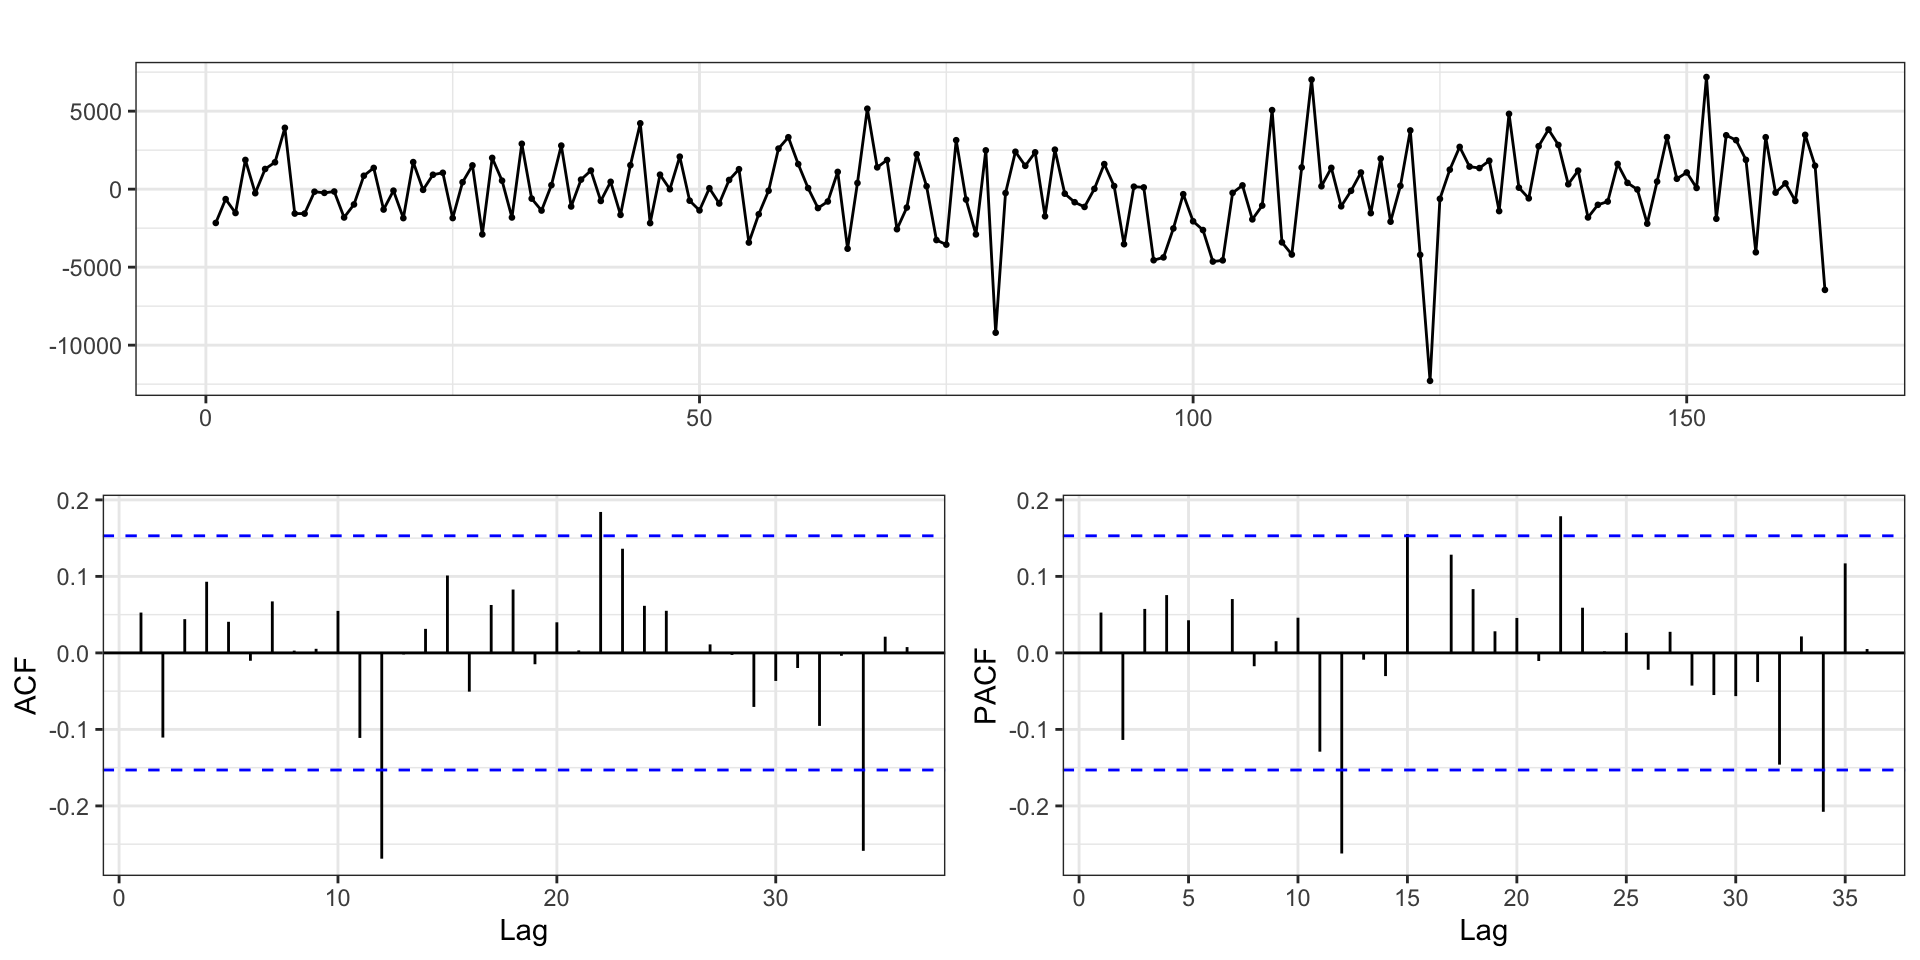
\includegraphics[width=\textwidth]{Lec21_files/figure-beamer/unnamed-chunk-17-1} \end{center}

\end{frame}

\hypertarget{random-projections}{%
\section{Random Projections}\label{random-projections}}

\begin{frame}{Low Rank Approximations via Random Projections}
\protect\hypertarget{low-rank-approximations-via-random-projections}{}

\begin{enumerate}
\tightlist
\item
  Starting with an matrix \(\underset{m \times n}{\symbf{A}}\).
\end{enumerate}

\pause

\begin{enumerate}
\setcounter{enumi}{1}
\tightlist
\item
  Draw a Gaussian random matrix
  \(\underset{n \times k+p}{\symbf{\Omega}}\).
\end{enumerate}

\pause

\begin{enumerate}
\setcounter{enumi}{2}
\tightlist
\item
  Form \(\symbf{Y} = \symbf{A}\,\symbf{\Omega}\) and compute its QR
  factorization \(\symbf{Y} = \symbf{Q}\,\symbf{R}\)
\end{enumerate}

\pause

\begin{enumerate}
\setcounter{enumi}{3}
\tightlist
\item
  Form \(\symbf{B}=\symbf{Q}'\,\symbf{A}\).
\end{enumerate}

\pause

\begin{enumerate}
\setcounter{enumi}{4}
\tightlist
\item
  Compute the SVD of
  \(\symbf{B} = \symbf{\hat{U}}\,\symbf{S}\,\symbf{V}'\).
\end{enumerate}

\pause

\begin{enumerate}
\setcounter{enumi}{5}
\tightlist
\item
  Form the matrix \(\symbf{U} = \symbf{Q} \, \symbf{\hat{U}}\).
\end{enumerate}

\pause

\begin{enumerate}
\setcounter{enumi}{6}
\tightlist
\item
  Form \(\symbf{\tilde{A}} = \symbf{U}\symbf{S}\symbf{V}'\)
\end{enumerate}

\vspace{2mm}

Resulting approximation has a bounded expected error,

\[ E| \symbf{A} - \symbf{U}\symbf{S}\symbf{V}'\|_F \leq \left[1 + \frac{4\sqrt{k+p}}{p-1} \sqrt{\min(m,n)} \right] \sigma_{k+1}. \]

\begin{center}
Halko, Martinsson, Tropp (2011)
\end{center}

\end{frame}

\begin{frame}{Random Matrix Low Rank Approximations and GPs}
\protect\hypertarget{random-matrix-low-rank-approximations-and-gps}{}

The preceding algorithm can be modified slightly to take advantage of
the positive definite structure of a covariance matrix.

\begin{enumerate}
\tightlist
\item
  Starting with an \(n \times n\) covariance matrix \(\symbf{A}\).
\end{enumerate}

\pause

\begin{enumerate}
\setcounter{enumi}{1}
\tightlist
\item
  Draw Gaussian random matrix
  \(\underset{n \times k+p}{\symbf{\Omega}}\).
\end{enumerate}

\pause

\begin{enumerate}
\setcounter{enumi}{2}
\tightlist
\item
  Form \(\symbf{Y} = \symbf{A}\,\symbf{\Omega}\) and compute its QR
  factorization \(\symbf{Y} = \symbf{Q}\,\symbf{R}\)
\end{enumerate}

\pause

\begin{enumerate}
\setcounter{enumi}{3}
\tightlist
\item
  Form the \(\symbf{B}=\symbf{Q}'\,\symbf{A} \, \symbf{Q}\).
\end{enumerate}

\pause

\begin{enumerate}
\setcounter{enumi}{4}
\tightlist
\item
  Compute the eigen decomposition of
  \(\symbf{B} = \symbf{\hat{U}}\,\symbf{S}\,\symbf{\hat{U}}'\).
\end{enumerate}

\pause

\begin{enumerate}
\setcounter{enumi}{5}
\tightlist
\item
  Form the matrix \(\symbf{U} = \symbf{Q} \, \symbf{\hat{U}}\).
\end{enumerate}

\pause

Once again we have a bound on the error,

\[
  E \|\symbf{A} - \symbf{U}\symbf{S}\symbf{U}'\|_F 
\lesssim c \cdot \sigma_{k+1}. 
\]

\begin{center}
Halko, Martinsson, Tropp (2011), Banerjee, Dunson, Tokdar (2012)
\end{center}

\end{frame}

\begin{frame}{Low Rank Approximations and GPUs}
\protect\hypertarget{low-rank-approximations-and-gpus}{}

Both predictive process and random matrix low rank approximations are
good candidates for acceleration using GPUs.

\vspace{3mm}

\begin{itemize}
\tightlist
\item
  Both use Sherman-Woodbury-Morrison to calculate the inverse (involves
  matrix multiplication, addition, and a small matrix inverse).
\end{itemize}

\vspace{3mm}

\begin{itemize}
\tightlist
\item
  Predictive processes involves several covariance matrix calculations
  (knots and cross-covariance) and a small matrix inverse.
\end{itemize}

\vspace{3mm}

\begin{itemize}
\tightlist
\item
  Random matrix low rank approximations involves a large matrix
  multiplication (\(\symbf{A}\,\symbf{\Omega}\)) and several small
  matrix decompositions (QR, eigen).
\end{itemize}

\end{frame}

\begin{frame}{Comparison (\(n=15,000\), \(k=\{100,\ldots,4900\}\))}
\protect\hypertarget{comparison-n15000-k100ldots4900}{}

\begin{center}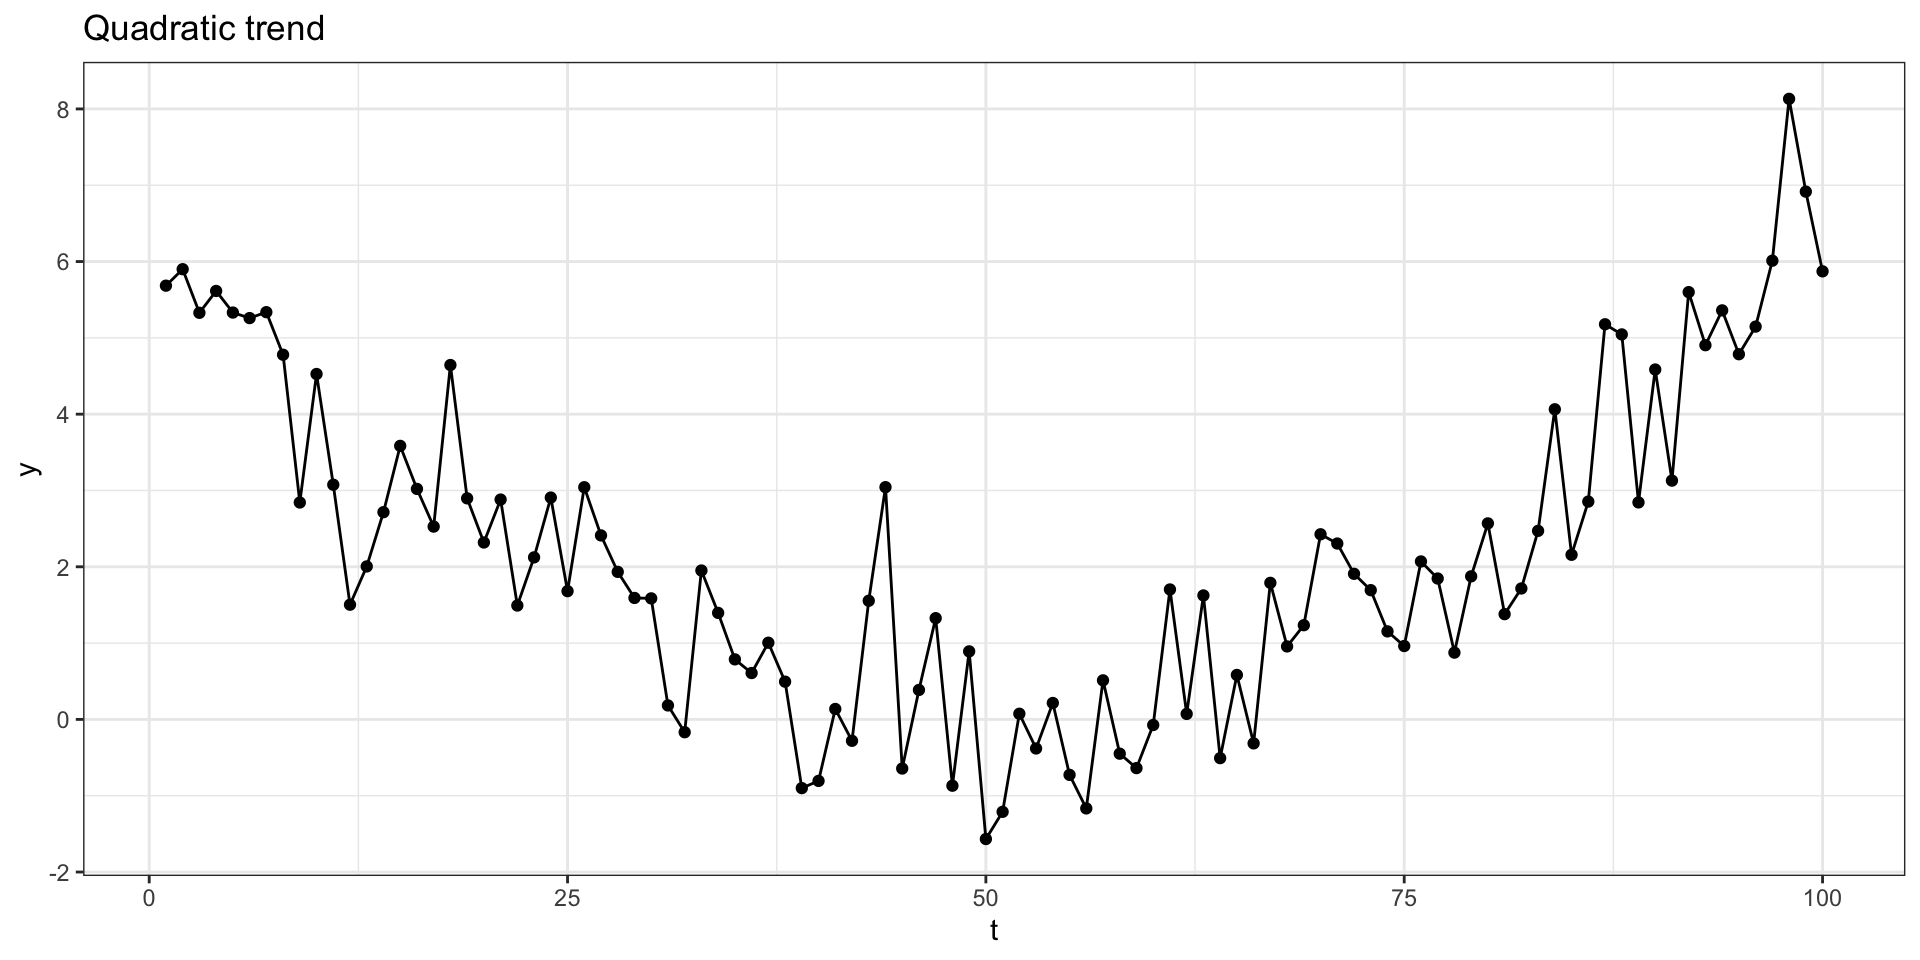
\includegraphics[width=\textwidth]{Lec21_files/figure-beamer/unnamed-chunk-18-1} \end{center}

\end{frame}

\begin{frame}[t]{Rand. Projection LR Depositions for Prediction}
\protect\hypertarget{rand.-projection-lr-depositions-for-prediction}{}

\small

This approach can also be used for prediction, if we want to sample

\[\symbf{y} \sim \mathcal{N}(0,\symbf{\Sigma})\] \[
\Sigma \approx \symbf{U} \symbf{S} \symbf{U}^t = (\symbf{U} \symbf{S}^{1/2} \symbf{U}^t)(\symbf{U} \symbf{S}^{1/2} \symbf{U}^t)^t 
\]

then

\[
y_{\text{pred}} = (\symbf{U}\, \symbf{S}^{1/2}\,\symbf{U}^t) \times \symbf{Z} \text{ where } Z_i \sim \mathcal{N}(0,1)
\]

because \(\symbf{U}^t \, \symbf{U} = I\) since \(\symbf{U}\) is an
orthogonal matrix.

\vvfill

\begin{center}
\footnotesize
Dehdari, Deutsch (2012)
\end{center}

\end{frame}

\begin{frame}{}
\protect\hypertarget{section-2}{}

\vspace{5mm}

\begin{center}
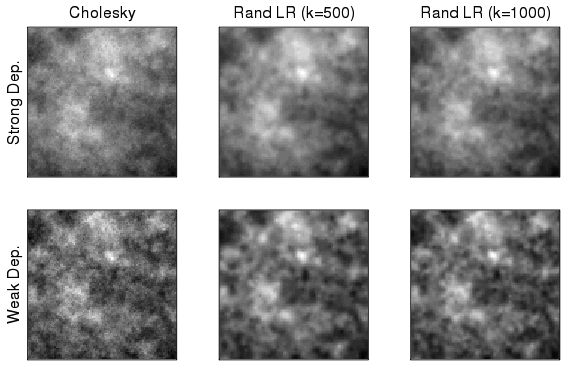
\includegraphics[width=\textwidth]{figs/RandLRPred.png}
\end{center}

\[ n=1000, \quad p=10000 \]

\end{frame}

\end{document}
